\documentclass[ProjectABM]{subfiles}
% WARNING: AuCTeX local variables only get reset when file is loaded
% and differ between this file and ProjectABM.tex
% so must re-load whichever file you want to compile with C-x C-v

% WARNING: Different AucTeX execution depending on whether
% 0. Being compiled as standalone document
%    * Compile main once
%    * Then compile this one
%    * Keep compiling until nothing changes
% 0. Being compiled as subfile of main document
%    * Just compile main document repeatedly

\providecommand{\econtexRoot}{}
\renewcommand{\econtexRoot}{..}
\providecommand{\econtexPaths}{}\renewcommand{\econtexPaths}{\econtexRoot/Resources/econtexPaths}
% The \commands below are required to allow sharing of the same base code via Github between TeXLive on a local machine and Overleaf (which is a proxy for "a standard distribution of LaTeX").  This is an ugly solution to the requirement that custom LaTeX packages be accessible, and that Overleaf prohibits symbolic links
\providecommand{\econtex}{\econtexRoot/Resources/texmf-local/tex/latex/econtex}
\providecommand{\econtexSetup}{\econtexRoot/Resources/texmf-local/tex/latex/econtexSetup}
\providecommand{\econtexShortcuts}{\econtexRoot/Resources/texmf-local/tex/latex/econtexShortcuts}
\providecommand{\econtexBibMake}{\econtexRoot/Resources/texmf-local/tex/latex/econtexBibMake}
\providecommand{\econtexBibStyle}{\econtexRoot/Resources/texmf-local/bibtex/bst/econtex}
\providecommand{\econtexBib}{economics}
\providecommand{\notes}{\econtexRoot/Resources/texmf-local/tex/latex/handout}
\providecommand{\handoutSetup}{\econtexRoot/Resources/texmf-local/tex/latex/handoutSetup}
\providecommand{\handoutShortcuts}{\econtexRoot/Resources/texmf-local/tex/latex/handoutShortcuts}
\providecommand{\handoutBibMake}{\econtexRoot/Resources/texmf-local/tex/latex/handoutBibMake}
\providecommand{\handoutBibStyle}{\econtexRoot/Resources/texmf-local/bibtex/bst/handout}

\providecommand{\FigDir}{\econtexRoot/Figures}
\providecommand{\CodeDir}{\econtexRoot/Code}
\providecommand{\DataDir}{\econtexRoot/Data}
\providecommand{\SlideDir}{\econtexRoot/Slides}
\providecommand{\TableDir}{\econtexRoot/Tables}
\providecommand{\ApndxDir}{\econtexRoot/Appendices}

\providecommand{\ResourcesDir}{\econtexRoot/Resources}
\providecommand{\rootFromOut}{..} % Path back to root directory from output-directory
\providecommand{\LaTeXGenerated}{\econtexRoot/LaTeX} % Put generated files in subdirectory
\providecommand{\econtexPaths}{\econtexRoot/Resources/econtexPaths}
\providecommand{\LaTeXInputs}{\econtexRoot/Resources/LaTeXInputs}
\providecommand{\LtxDir}{LaTeX/}
\providecommand{\EqDir}{Equations} % Put generated files in subdirectory


\onlyinsubfile{% https://tex.stackexchange.com/questions/463699/proper-reference-numbers-with-subfiles
    \csname @ifpackageloaded\endcsname{xr-hyper}{%
      \externaldocument{\econtexRoot/BufferStockTheory}% xr-hyper in use; optional argument for url of main.pdf for hyperlinks
    }{%
      \externaldocument{\econtexRoot/BufferStockTheory}% xr in use
    }%
    \renewcommand\labelprefix{}%
    % Initialize the counters via the labels belonging to the main document:
    \setcounter{equation}{\numexpr\getrefnumber{\labelprefix eq:Dummy}\relax}% eq:Dummy is the last number used for an equation in the main text; start counting up from there
}


\onlyinsubfile{\externaldocument{ProjectABM}} % Get xrefs -- esp to appendix -- from main file; only works properly if main file has already been compiled;

\begin{document}

% Attempted to make all lines used for Web version contain {Web} (or version with only single curly brace at end) so can be removed with sed
\providecommand{\versn}{pdf} % Version; like, web or pdf or journal submission
\ifthenelse{\boolean{Web}}{    % {Web}
  \renewcommand{\versn}{Web}     % Too hard to figure out passing -output-directory through make4ht through htlatex, so web version is compiled with junk files in main directory
  \renewcommand{\rootFromOut}{.} % {Web}
}{}  % {Web}

% Tiny info header at top to track git commit
%\hfill{\tiny \jobname~\versn~\today~{at} \DTMcurrenttime, \input{\ResourcesDir/.git-source-commit}~~\input{\ResourcesDir/.git-public-commit}}

\title{Equity Premium Puzzle, Expectations and Covid-19:\\ Evidence from Germany}

\author{Adrian Monninger\authNum}

\keywords{equity premium puzzle - participation cost - adjustment costs - expectations - Covid-19}

\jelclass{D14, G11, G5}


\renewcommand{\forcedate}{February 7, 2022}\date{\forcedate}

\maketitle
\hypertarget{abstract}{}
\begin{abstract}
	What differentiates households who invest in financial assets from those who do not? I ask respondents directly using the Bundesbank Online Pilot Survey on Consumer Expectations in Germany about the reasons for their investment decisions during the Covid-19 pandemic. I find that lack of information and interest are the biggest determinants for non-participation, while risk and time constraints prevent households to re-balance. Buyers invest either because of expected increasing asset prices or due to a (pre-existing) savings plan. Additionally, I find that the probability to be a buyer depends highly on stock price expectations. Conversely, households who have higher expectations of property prices as well as inflation are less likely to buy financial assets.
%What prevents households from investing in financial assets and what makes them overcome these factors? This paper asks respondents directly about the reasons for their decisions during the Covid-19 pandemic. Using the Bundesbank Online Pilot Survey on Consumer Expectations, I find that lack of information and interest are the biggest determinants for non-participation, while risk and time constraints prevent households to re-balance. Buyers invest either because of expected increasing asset prices or due to a (pre-existing) savings plan. Additionally, I find that households who have higher expectations of property prices as well as inflation are less likely to buy.
\end{abstract}


% Various resources
\hypertarget{links}{}

\begin{authorsinfo}
  \name{Contact: \href{mailto:amonnin1@jhu.edu}{amonnin1@jhu.edu}, Department of Economics, Johns Hopkins University, Baltimore, MD 21218}
\end{authorsinfo}

\newcommand{\thankstext}{
I am deeply indebted to the members of the Deutsche Bundesbank BOP team, in particular Tobias Schmidt, Stefan Ried, Olga Goldfayn-Frank, and Misina Cato, as well as Chris Carroll, Johannes Stroebel, Annette Vissing-Jorgensen and my fellow students from the Johns Hopkins University. All errors are my own.}

\ifthenelse{\boolean{Web}}{}{
  \begin{minipage}{0.9\textwidth}
    \tiny \thankstext
\end{minipage}
} % {Web}
{\titlepagefinish}

\hypertarget{Introduction}{}
\section{Introduction}\label{sec:intro}

%\paragraph{Many theories to explain equity premium puzzle}
The equity premium puzzle documents the small number of financial asset holders given the excess return these assets yield. While this is not a new phenomenon, the literature is still growing. Household finance papers have tested empirically a variety of factors why households do not hold stocks at all and if they do, why the fraction of their portfolio is so small. These mechanisms are usually tested individually using different time periods, locations, and reference groups which makes a comparison almost impossible.
%The equity premium puzzle is not a new phenomenon, but a vibrant one. Household finance papers have tested empirically a variety of factors why households do not hold stocks at all and if they do, why such a small share of their portfolio. These factors are usually tested one by one using different time periods, locations, and reference groups which makes a comparison almost impossible.

A comparison gets even harder when multiple circumstances change simultaneously. The Covid-19 pandemic offers such a period where stock markets fell dramatically and recovered vastly. Additionally, restrictions altered work, consumption, and leisure patterns.

%\paragraph{This paper: high level summary}
 To overcome this identification problem, I ask households directly about their financial asset investments they made during the first six months of the pandemic and the factors that led to their decision. 
 Using novel data from the Bundesbank Online Panel (BOP) allows me to distinguish between non-participants, households who did not adjust their portfolio, as well as buyers and sellers. Each type ranks various reasons brought forward in the literature from very important to not important at all. Hence, I can assess which factors were more or less important and how they relate to each other. 
 Additionally, the survey includes various questions on household expectations. Hence, I can analyze how they affect financial behavior.
 %to assess factors which played a role in their financial investment decision. %\textit{What are the most important factors of the equity premium puzzle?} With the natural follow up question \textit{And what makes households overcome them?}

%\paragraph{Contributions:}
%The contributions of this paper are threefold. Firstly, I can compare the importance of many factors and assess how they correlate with each other. Secondly, while most papers focus on the participation part, I ask why households did not adjust their portfolio, or if they did what drove their decision. Lastly, I can link financial asset investment decisions with expectations about macro-variables.

%\textbf{VS}

%\paragraph{Gap In the Literature}
This paper contributes to three gaps in the literature. First, it compares magnitudes or importance of participation costs. Here, it is close to \cite{choi_2020} who ask in 2016 around 1,000 household heads what determines their portfolio equity share. One important difference to this paper is that while they ask for general factors, I focus on reasons concerning a fixed 6 months period which makes it more concrete and therefore more accessible to answer in a survey setting. %Other papers focus on wealthy investors (eg \cite{bender_et_al_2019}). 

Second, adjustment costs which need to be paid when changing the portfolio are crucial when matching shares invested in equity markets. Papers such as \cite{giglio_et_al_2019five} advocate for a fixed exogenous proportion of households who re-balance each period. Alternatively,  \cite{bonaparte_et_al_2012adjustment} model them as a proportion of income. Nevertheless, there is no clear structural model nor convincing empirical evidence explaining what these adjustment costs consist of. My survey questions allow me to ask households explicitly what prevents them from adjusting and what makes them decide to buy or sell.

Third, the literature connecting financial asset decisions and expectations focus on expected stock market returns and equity investments. For example, \cite{arrondel_et_al_2014subjective_return_expectation} find that participation increases monotonically with stock market expectations and \cite{choi_2020} show that expected higher returns are very or extremely important by a quarter of all stock market participants. %\textbf{NOTE TO ME: ADD MATEO WHEN READY}.
 Additionally, \cite{giglio_et_al_2019five} find empirical evidence for wealthy retail investors. In contrast to the literature, I shift attention towards inflation and house prices whose influence on financial asset decisions is more explorative. %stock market participation and other macro-variables such as inflation and house prices.

% \begin{itemize}
	%     \item Asking directly many mechanisms
	%     \item Not only participation, but why bought, sold, not adjust
	%     \item Expectations: Not only about stock market expectation, but other macro variables
	%	  \item In context of Covid
	% \end{itemize}

%\paragraph{My Results}
My findings are that lack of information and lack of interest are the most important factors why households do not participate in financial markets. Reasons can be grouped into risk aversion, lack of resources, and savings, whereas the first two have a life-cycle and the latter an income component. Second, households did not adjust their existing portfolio either because they thought it is a bad timing or due to time constraints. Third, households invested either because they expected higher stock market prices - which is related to other factors such as time, information, and peer effect - or due to a (pre-existing) savings plan. Additionally, households are more likely to invest in assets they're already holding. Fourth, some households sold to re-balance or prevent further losses. Finally, households are less likely to buy financial assets if their expectations of house prices as well as inflation is higher. Conversely, higher expected stock market prices increases the probability to be a buyer.

%\begin{enumerate}
%	\item No participation:
%	\begin{itemize}
%		\item lack of information and interested most important, before risk factors
%		\item 3 components: risk aversion, lack of resources, no savings
%		\item first 2 lifecycle component, last income component
%	\end{itemize}
%	\item No Adjustment
%	\begin{itemize}
%		\item Market is too risky/uncertain atm
%		\item 2 components: bad timing and lack of time
%		\item needs to get further attention
%	\end{itemize}
%	\item Bought
%	\begin{itemize}
%		\item Good starting point or had a savingsplan in place
%		\item First time buyers: more time
%		\item Bought same asset type
%	\end{itemize}
%	\item Sold
%	\begin{itemize}
%		\item cash out or rebalancing
%		\item some are driven out
%	\end{itemize}
%	\item Expectations
%	\begin{itemize}
%		\item Houseprices crowd out financial asset investments (Owner and renter)
%		\item Higher inflation expectations reduces likelihood to buy
%	\end{itemize}
%\end{enumerate}
% \begin{itemize}
	%     \item 50\% no participation, 25\% participated, but did not adjust and 25\% adjusted their portfolio.
	%     \item Demographics which increased the probability to buy stocks are: education (college graduates), sex (male), wealth (higher income), age (being younger than 30)
	%     \item Reasons no participation: 70\% agree that lack of information and no interest is important, 60\% distrust, time constraints and peer-effects
	%     \item By demographics: variation can be captured by cohort effects; female are less interested
	%     \item Reasons un-adjusted: too risky, high valuation and no time most important
	%     \item By demographics: no additional savings and peer-effect captured by cohort effects. The three above are relatively constant
	%     \item Reason bought: low valuation and saving plan are very important
	%     \item first time buyers: time played a role
	%     \item bought and sold: low valuation and additional information, but less likely a savings plan
	%     \item Reason sold: high valuation and re-balancing most important, some sold due to uncertainty and shock
	%     \item Buy asset types: funds and bonds most prominently held. Re-balancing from funds towards bonds. Mostly bought asset type they already held
	%     \item Buy and Expectations: more likely to buy if think gdp increases stronger and lower if property prices increase stronger. Counter-intuitively, probability increases when unemployment is expected to increase %could be due to: If updated expectations on any variable, more likely to buy: Updating and additional information effect. Could hold for unemployment rates as well (was heavily in the news)
	% \end{itemize}

% No insights in:
% \begin{itemize}
	%     \item Value bought (tried, reg, tobit, heckman); also ratio income not much. Might be something with reasons (low valuation and more income is important, plan and time not)
	% \end{itemize}


%\paragraph{Equity premium puzzle}


%\paragraph{Why 2020? Aka my short Literature review}
The year 2020 is an interesting time period to study. Due to Covid-19 and corresponding restrictions in March 2020, the German stock market (DAX) plummeted by almost 40\%, but recovered vastly and finished with a yearly return of 3.5\%. Nevertheless, the overall participation rate increased by 2.7 million. The \cite{DAI_2021} reports that the biggest increase (40\%) was made for Germans younger than 40. %\textbf{Note to me: Add PAPI if ready}

% DAI 2021: 
% \begin{itemize}
	%     \item 12.4 mio people own financial assets/ 1/6 above 14
	%     \item in 2020: 
	%     \begin{itemize}
		%         \item 2.7mio more
		%         \item 1 mio younger than 40
		%         \item 14-29 years: +67\%
		%         \item 30-39 years: +34\%
		%         \item <40: +40\%
		%     \end{itemize}
	% \end{itemize}

% Add numbers of other countries?!

Economic theory gives many explanations how this period could have impacted financial investment decisions. On the one hand, the bufferstock model by \cite{carroll2009bufferstock} suggests that higher income uncertainty increases the target level of wealth to dampen possible shocks. %While it is not clear, whether households should invest in the stock market, it is definetely one possibility. 
Additionally, a bust is usually followed by a recovery which marks a good opportunity to start investing. Hence, households with more optimistic views should invest. Lastly, Covid-19 affected everyday life in many dimensions. Consumption restrictions could have increased savings and free time for some households which could be used to organize personal finances. 
%Of course, this experience is extremely heterogeneous, as working remotely and home schooling marked a huge burden on families with small children.

On the other hand, multiple paper provide evidence why stock market participation should fall after Covid-19. \cite{malmendier_2011} would argue that the vast decline in stock prices scares people away. This should affect especially younger households who put more emphasis on recent periods when making financial asset decisions. Additionally, the path of recovery contains a lot of uncertainty as it depends on behavior of others and government, vaccination availability and efficacy, as well as possible mutations. All these risk assessments are reflected in the stock market, hence, workhorse models such as Capital Asset Pricing Models (CAPM) suggest that people would reduce their asset holdings. Lastly, working remotely and home schooling urged households to additional consumption (e.g digital infrastructure) and marked a huge burden especially on families with young children. For them, the pandemic could have a negative effect on financial asset holdings.

% This increase can have many sources. 
% LITERATURE SUMMARY ABOUT FACTORS RELEVANT IN 2020

% Covid-19 affected everyday life and the economy in many dimensions. Firstly, after restrictions in March 2020, stock market prices fell vastly. \cite{malmendier_2011} would argue that this experience scares people away

% \begin{itemize}
	%     \item Show graphs of stockholding puzzles (HFCS, SCF)
	%     \item Show fall and sore of stock markets after Corona (compare with 2008?) 
	% \end{itemize}
% Stories:
% a) Factors which could decrease stock holdings: 
% i) shock: scared people away (Malmendier and nagel)
% ii) Which recovery? V,L,W,K? Leads to higher uncertainty

% b) Factors which could increase stock holdings:
% i) Higher uncertainty leads to higher savings (Bufferstock Carroll)
% ii) After crises low valuation which makes it a good opportunity to invest
% iii) Covid specific factors: consumption restrictions (more savings for some) and more time (for some)



% \paragraph{My research question}

% \paragraph{My Data}



%\paragraph{Data + Survey Methodology}
This richness of mechanisms makes it nearly impossible to identify the importance of each factor individually. Therefore, I ask respondents directly which reason played a crucial role in their decision making process. The BOP asks to a representative sample of around 2,000 German households questions about expectations of macroeconomic variables, personal income and consumption. In August 2020, I included 3 to 6 questions for each respondent with whom I can group households into four types. Between March 2020, which marks the beginning of Covid-19 restrictions, and August 2020, respondents could have either i) not participated in financial asset markets ii) not adjusted their portfolio, iii) bought, or iv) sold assets. Each type receives a set of reasons which could be influential in their decision. The task is then to rank each factor from very to not important.

Asking households directly is appealing in this context as importance of individual factors can be identified. Therefore, it assumes that answers can be trusted and respondents are aware of their \textit{true} decision making process.\footnote{See \cite{choi_2020} for a brief discussion about survey methodology.} While these assumptions might not hold for all respondents, a general ranking order of factors might still be valid and informative.
% Asking households directly are appealing in this context to compare the mechanisms, but have weaknesses. \textbf{ADD THEM HERE: PROS AND CONS}

% \cite{choi_2020}: 'Survey methodologies, of course, have weaknesses. Survey respondents might not be highly motivated to give accurate responses, and the meaning of each response category (e.g., “very important”) probably differs across respondents. However, to the extent that such measurement error is white noise, the ordinal ranking of importance and agreement ratings will still be informative.More fundamentally, individuals might not know the true motivations for their decisions because they have not introspected seriously enough, their memory has faded, or they were subliminally influenced. A related critique is the argument that respondents may not regard a factor as important but nonetheless invest “as if” it were (Friedman (1953)). Under this view, the fact that an assumption is false is unimportant as long as it generates accurate predictions.' \textbf{Methodology: Survey Weaknesses}

% \cite{choi_2020}: '1. perceptions are unlikely to be entirely unrelated to true decision-making process 2. choose between theories that have similar predictions for prices and quantities but very different implications for our understanding of the world 3. individuals’ perceptions of their decision-making process affect how they forecast their future actions, which itself is an input into their actions today 4. these perceptions can affect an individual’s demand for debiasing mechanisms, information, and advice 5. we believe that it is inherently interesting to know what individuals believe about themselves and the reasons for their behavior. Barberis et al. (2015) argue that theory should endeavor to match survey measures of investor beliefs.' \textbf{Why surveys are a good idea}

%\paragraph{Rest of Paper}
The rest of the paper is structured as follows. First, Section \ref{sec:literature} summarizes the literature on drivers of financial decisions as well as household expectations. Afterwards, section \ref{sec:data} discusses the questionnaire and describes the data. The core section \ref{sec:results} analyzes the role of factors and expectations on financial asset decisions. Lastly, section \ref{sec:robustness} assesses generality of the results and section \ref{sec:conclusion} concludes.

%\hypertarget{The-Problem}{}

\section{Literature Review}\label{sec:literature}
%\textbf{Keep for now, maybe erase later}

%\paragraph{Intro}
This paper builds upon two large literature strands; the equity premium puzzle and the growing expectations literature.

%\paragraph{Equity Premium puzzle in general}
The equity premium is defined as the excess return on financial assets to the riskfree rate. Given this, economic models cannot rationalize the low number of stock holders using \textit{reasonable numbers} for relative risk aversion parameters (See \cite{mehra_porescott_1985equity_premium, haliassos_bertraut_1995equity_premium} for early discussions and \cite{Gomes_et_al_2021} for a recent literature review).\footnote{ The actual size depends on measurement, time and space (see\cite{vanEwijk_et_al_2012meta_equity_premium} for a meta analysis)} The puzzle is twofold. First, the low participation in the stock market (intensive margin) and second, the relative low share of risky assets of total portfolio (extensive margin) \citep{campbell_2006household_finance}. The literature accumulated various factors which can be grouped in two categories: risk and participation costs. %, and social interaction. Social Interaction or lack of such is a participation cost...

%\paragraph{Risk}
One explanation focuses on risks faced by households. In particular, the correlation between labor income and stocks can limit participation (e.g.,\cite{BCG2007stocklabor}). Other background risks such as housing \citep{cocco2005housing} or health \citep{GJT1996_health} reduce stock holdings as well. Nevertheless, \cite{catherine2020_countercyclical} argues that renters do have larger idiosyncratic income risk which reduces their stock market participation.% especially of renters while \cite{brandsaas2021_housing} finds that households liquidate financial assets to seize home ownership. \textbf{Cool papers, but misplaced here?}

When it comes to stock market risks, workhorse models such as Capital Asset Pricing Model (CAPM) argue that through macroeconomic shocks, market volatility increases which decreases the share households want to invest in risky assets. Additionally, \cite{malmendier_2011} argue that experiencing stock market crashes can have long lasting effects on financial risk taking behavior and find evidence in the US. A similar study by \cite{ampudia_ehrmann_2017macroeconomic} uses European data and confirms the results. 
%Additionally, a macroeconomic shock can also boost uncertainty. Workhorse models such as CAPM argue that an increase in volatility, should decrease the savings households put in the stock market.

%\paragraph{Participation Costs}
As these risk factors are not enough to match empirical moments, another venue imposes a small participation cost for everyone who wants to enter equity markets (e.g \cite{vissing_2003, HM2003portfolio, GM2005portfolio}). The idea is that financial asset decisions are costly and only a fraction of households are willing to pay that price. While direct costs such as setting up a brokerage account only make a small part of it, a large literature explores indirect costs. The latter concerns psychological costs or barriers which need to be overcome. While these cannot be directly paid with money, the household has to allocate time and effort which could have been spent otherwise on more pleasant things. While these are not \textit{costs} in the narrow sense, but should be more thought of as \textit{barriers} or \textit{opportunity costs}, I still will refer to them as such.


%\paragraph{Information, Awareness and Financial Literacy}
%Information costs received early attention. 
An early study by \cite{king_leape_1987asset} uses the Survey of Consumer Financial Decisions and shows that more than one third of non-participants argue that `they did not know enough about it' as a reason of their non-participation. These information costs can consist of unawareness of financial products, differences within them, how financial markets work and how to invest. % such as different stocks and funds and financial literacy. 
For the former, \cite{guiso_jappelli_2005} find that socioeconomic variables such as education, wealth, income, year of birth, as well as long-term bank relations, social interaction and newspaper readership increases the awareness which then leads to a higher probability of stock market participation. 

Regarding financial literacy, \cite{lusardi_mitchell_2011financial_literacy} show that many households lack knowledge of basic economic principles. Drivers are education, gender, race, and location. %This is particularly true for, persons which are lower educated and women are less financial literate. % which leads to lower stock market participation. In an overview, they report that women are less financially literate -- which leads to lower stock holding participation (\cite{almenberg_2015gender}) -- and higher educated are also more financial literate. Additional factors are ethnic/racial and regional differences. 
Several papers show the strong link between financial literacy and stock market participation. For instance, \cite{guiso_japelli_2002household_book} use Italian data, \cite{hochguertel_et_al_2002household,vanrooij_et_al_2011} Dutch and \cite{borsch_eymann_2000household} German data.

%\paragraph{Time: Opportunity Costs}
Gathering information about financial products, making the decision, and implementing it takes time. Hence, the opportunity cost of doing so is either work or leisure. \cite{bonaparte_et_al_2012adjustment} models the adjustment of one's portfolio as a proportion of income. Nevertheless, \cite{choi_2020} find that time constraints play only an important factor for 3\% of nonparticipants. %Nevertheless, this factor might not be easy to capture in survey questions.

%\paragraph{No interest: Cost of thinking about it (disutility)}
Additionally, thinking about ones finances might even entail additional disutility. \cite{shapiro_burchell_2012} highlight the importance of `financial anxiety' or `phobia' as a driver of financial illiteracy. \cite{choi_2020} report that in the US 37\% of nonparticipants stated that `not liking to think about one's finances' was a very or extremely important factor of their non-stock holding. Hence, allocating time into these decisions can be even more costly than opportunity costs.



%\paragraph{Trust/Sociability/Peer Effect}
%\cite{georgarakos_pasini_2011} summarizes another channel regarding trust and sociability. 
%A related channel concerns trust and peer effects. Trust is studied by \cite{guiso_et_al_2008trusting} who show that households with lower trust in other people are more afraid of being cheated on which lowers the expected payoffs from stock holdings.
On the contrary, social interaction and peer-effects can lower participation costs. %on stock market participation gained much attention (e.g. \cite{georgarakos_pasini_2011, brown_2008, hong_et_al_2004social}).
The mechanism is that gaining information is costly and `word-of-mouth' communication can lower these costs \citep{brown_2008}. Additionally, \cite{hong_et_al_2004social} argue that individuals have pleasure in discussing recent stock markets dynamics and choose it as a casual conversation topic. Examples of these effects on stock market behavior are plenty and consist of parental transmission \citep{CS2000_parental}, workplace \citep{duflo_saez2002_workplace}, neighbors and church communities \citep{hong_et_al_2004social, brown_2008}.

%\textbf{Rewrite:} Following \cite{georgarakos_pasini_2011} who uses the classification by \textbf{Durlauf and Fafchamps' (2004)}, the difference between the two is that interpersonal trust, sharing and reciprocity, while the latter focuses social networks or civic engagement. \textbf{No one cares}



%\cite{choi_2020}: 'Second, we ask about the importance of having intended to invest in stocks but simply not having gotten around to it (''intended to invest in stocks but never got around to it''), perhaps due to tie-inconsistent procrastination (Laibson (1997), O'Donoghue and Rabon (1999))'. \textbf{Time}

%\cite{choi_2020}: 'the lest important factor is delay despite an intention to invest in stock (3\% of nonparticipants). Prior evidence shows that individuals' financial choices exhibit considerable inertia (Samuelson and Zeckhauer (1988), Choi et al. (2002, 2004)), but people do eventually move away from their status quo to what they perceive to be their optimum (Carroll et al. (2009)), even if it takes them a few years. Therefore, in a sample that includes many middle-aged and older adults, it may not be unexpected that procrastination is a relatively small determinant of stock market nonparticipation.' \textbf{Time}


%Adjustment Cost
%In addition to participation costs, households face adjustment costs when they change their portfolio. Models without them tend to match participation rates, but predict a portfolio share in financial assets of close to 100\% (Coco and Gomes?). \cite{bonaparte_et_al_2012adjustment} models them solely as a proportion of income, but the literature on assessing it empirically is scarce.

%\cite{bonaparte_et_al_2012adjustment}: 'the cost of trading stocks takes a particular form: a proportion of income. As noted, this captures a time cost of trading' \textbf{Time and Adjustment} $\to$ should the reason increase importance with income? Alternatively: if richer, more likely to have some advisor...


% \paragraph{Personal Values/Moral}
% Lastly, personal values or moral issues can prevent households from holding stocks. \cite{kaustia_2011} argue that personal values determine investment decisions and individuals have a taste for different investment goods (similar to consumption goods). While this can just lead to a preferred asset type, 'stock market aversion' can also appear due to a cognitive dissonance between personal values and actions. Hence, individuals might not want to invest.

%\paragraph{Expectations and Stock Market Participation}
The second class of literature focuses on expectations of traders/ households and their financial asset investments. This paper relates to stock market return, inflation, and house price expectations.

%\textbf{Return expectations}
\cite{arrondel_et_al_2014subjective_return_expectation} find that participation among households increases monotonically with stock market expectations and \cite{choi_2020} show that expected higher returns are very or extremely important by a quarter of all stock market participants. For wealthy retail investors, \cite{giglio_et_al_2019five} confirm the mechanism.

%\textbf{Inflation}
The effect of expected inflation and the probability to buy financial assets is less clear. Empirically, higher inflation can have a short-term negative impact on stock prices, but a possible positive long term effect (eg \cite{anari_kolari_2001inflation}). \cite{campbell_vuolteenaho_2004inflation} list three reasons for a negative short-term correlation. Firstly, inflation itself, or nominal interest rate increases by central banks, decreases profitability of companies. The former can be explained by sticky prices meaning that not all companies can adjust their prices while the latter means higher lending costs for capital. Secondly, periods of higher inflation have also higher risks which investors might not like and thirdly, investors might fail to adjust the decomposition of nominal prices into constant real rates and increasing inflation which leads to an undervaluation in high inflation periods \citep{modigliani_cohn1979inflation}.

Nevertheless, the question how households react to higher inflation expectations can have other reasons. For instance, \cite{CCG_2020_inflation_communication} find that households have a \textit{stagflationary view} and connect inflation with a negative impact on the economy. This contrasts the classic Phillips Curve thinking of professional forecasters, where high inflation correlates with low unemployment and high output. %(Kamdar 2018)

%\textbf{Malmendier Handbook chapter: Inflation expectation: Strong evidence on influence on financial choices: homeownership (buy vs rent), mortgage borrowing, mortgage type (frm/arm)... Limited evidence on economic choices such as consumption, labor supply, wage negotiations}

%\textbf{House-prices and stock market}
Furthermore, this paper analyses the relationship between financial asset decisions and expectations of house prices. \cite{sutton2002houseprices} analyze house price changes as a response to a shock in equity prices. They find that in the US, UK, Canada, Australia, Netherlands, and Ireland a 1\% increase in equity prices leads to a 1 to 10\% higher house prices within 3 years. They rationalize the finding with an increase in housing demand due to a wealth effect on equity prices and that the stock market reflects expectations of national income. Nevertheless, they conjecture that in the US, stock market investments might be a substitute for housing assets and finds that in years of high investments in equity markets, demand of housing decreases. %Crowding out

\cite{cocco2005housing} shows that household finance models with housing can explain the lower share of equity holders as households who already invested in housing have limited resources to invest in the equity market. Additionally, house price risks lead to a crowding out effect of stock holdings.


%Correlation house prices and stock market:
%\textbf{Sutton 2002}: higher stockprices lead to higher house prices: 

%Expectations and other variables:
%\textbf{Kuchler Handbook chapter: House price expectation and buying}

%House prices and household investment:
%a) crowding out
%b) investing rather in housing than equity


%\textbf{TBD: ADD OTHER PAPERS}

\section{Data}\label{sec:data}

The data source of this paper is the \textit{`Bundesbank Online Pilot Survey on Consumer Expectations'} (BOP)\footnote{This paper uses data from the Bundesbank Online Pilot Survey on Consumer Expectations. The results published and the related observations and analysis may not correspond to results or analysis of the data producers.}, which is a monthly survey conducted by Deutsche Bundesbank since April 2020\footnote{The pilot phase covers the months April to June 2019, see \cite{bundesbank_2020} for details.}. A representative sample of around 2,000 German households per wave report their expectations about the development of inflation, house prices and interest rates in Germany as well as their past and planned expenditures and socio-demographic characteristics. In addition to questions which are asked on a regular basis, each wave has room for specific research questions.

\subsection{Key Variables}
In August 2020 (wave 8), households were asked three to six questions regarding their stock market behavior.\footnote{The complete questionnaire can be found in the appendix \ref{sec:ApndxQuestionnaire} or at \href{https://www.bundesbank.de/en/bundesbank/research/survey-on-consumer-expectations/questionnaires-850746}{Bundesbank website}.} Figure \ref{fig:timeline} shows the survey timeline. Firstly, respondents are asked if they held any financial assets (stocks, bonds, funds, others\footnote{The questionnaire contains info boxes about each asset type.}) actively in their portfolio prior to the Covid-19 pandemic. In case one of these questions is affirmed, the amount can be selected as a categorical variable. Secondly, I document their behavior between March and August. Here, respondents report whether they bought, sold or left their portfolio unchanged with a follow up question about the market value of these changes. %\textcolor{orange}{Reasons for this 6 month period only! Others eg \cite{choi_2020} does ask factors in general. Time bias (what is actually important and what used to be important) or what you think used to be important in the past. Also no savings or no time can be quiet seasonal. Same for shocks (its the corona shock) and the 2020 uncertainty...}

Based on the answers, respondents could belong to one of four types: \textit{no participation} (if they had no stocks before and haven't bought any), \textit{no adjustment} (if they had stocks before, but haven't adjusted their portfolio), \textit{bought} (if they bought during the period), and/or \textit{sold} (if they sold during the period). Each type receives a specific set of additional question with possible reasons for their behavior. Here, individuals are asked to rank the reasons on a four point scale from strongly agree to strongly disagree\footnote{The order of the answers is generated randomly for each respondent to avoid that scores depend on the order of question.}.

%\textbf{TBD: Data treatment}

For analyzing the responses I either use indicator variables which are one if the reason is above the respondents average of all factors. Alternatively, I follow \cite{choi_2020} and construct a standardized variable ($Z_i$) based on the formula:

\begin{verbatimwrite}{\EqDir/Standardization}
	\begin{align}
		Z_i = \frac{X_i - \Bar{X}}{\sigma}  \label{eq:standardization}
	\end{align}
\end{verbatimwrite}
	\begin{align}
		Z_i = \frac{X_i - \Bar{X}}{\sigma_i}  \label{eq:standardization}
	\end{align}


using mean ($\Bar{X}$) and standard deviation ($\sigma$) of all answers of one respondent. The advantage is that each reason becomes more comparable within and across observations as the standardization takes care of the fact that perception of `agreement' might differ among participants. Additionally, observations where all answers receive the same score are filtered out. These do not add any value and might even be a sign of low motivation and quality of the response.
 
%\begin{figure}
%	\centering
%	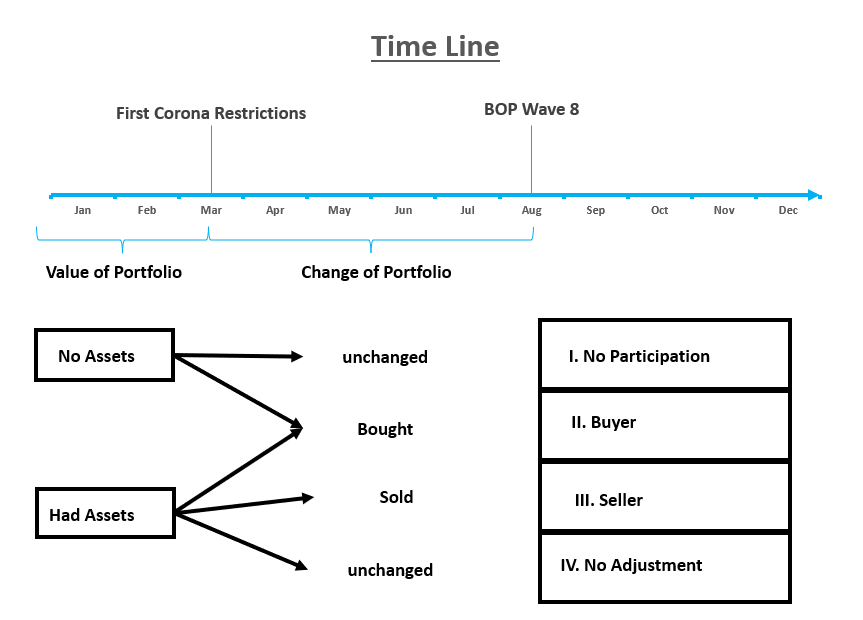
\includegraphics[width = \linewidth]{\FigDir/timeline.png}
%	\caption{Time Line of the Questionnaire}
%	\label{fig:timeline}
%\end{figure}

\begin{figure}[ht]
  \centerline{
    \includegraphics[width=6.0in]{\FigDir/Timeline}
  }
  \caption{Types of Equity and Non-Equity Holder} \label{fig:Timeline}
%\centerline{See Table~\ref{table:Calibration} for Numerical Values of Nodes Under Baseline Parameters}
\end{figure}


% 
        
        \node (NoAssets) [startstop] {Had no Assets};
        \node (HadAssets)[startstop, below of = NoAssets]{Had Assets};
        \node(Nopart)[startstop, right of = NoAssets, yshift = 2cm, xshift = 2cm]{I. Non-Participation};
        \node(Bought)[startstop, below of = Nopart,]{II. Bought};
        \node(Sold)[startstop, right of = HadAssets, xshift = 2cm]{III. Sold};
        \node(Noadjust)[startstop, below of = Sold, yshift = 1cm]{IV. No Adjustment};
        \draw[arrow](NoAssets) |- (Nopart);
        \draw[arrow](NoAssets) |- (Bought);
		\draw[arrow](HadAssets) |- (Bought);
		\draw[arrow](HadAssets) |- (Sold);
		\draw[arrow](HadAssets) |- (Noadjust);        %xshift and yshift
         %delete later

\subsection{Expectation data}
The BOP is rich in consumer expectations questions. It asks households about various macroeconomic variables in multiple formats. This paper exploits expected house prices and inflation and their role on buying financial assets. For both variables, respondents provide a qualitative statement, as well as a point estimate. Additionally, for inflation, respondents have to fit a distribution. Asking the same question in a different format increases robustness, as survey answers might differ substantially \citep{potter_et_al_2017prob,diercks2021asymmetric}.

For house prices, the BOP asks how rents and property prices in the area of the respondent change over the next 12 months. Options to answer range from decrease significantly to increase significantly with 5 steps. The point estimate is not bounded, but I winsorize the answers to 95\% in order to erase outliers.

The same holds true for inflation expectations. For the qualitative indicator, I add questions concerning `lending rates' and `fuel prices' as they all relate to price increases. For the probabilistic inflation expectation, households have to allocate 100\% into 10 bins ranging from deflation will be 12\% and higher to inflation will be 12\% and higher. In line with \cite{engelberg_manski_2009distribution} I fit either a generalized beta, triangular or uniform distribution.\footnote{Sample code can be found in \href{https://github.com/AMonninger/DensitySurveyEstimation}{GitHub}. Thanks to Tao Wang for sharing and collaborating.} As a result, I calculate mean, standard deviation, and 90-10 percentile spread to assess magnitude and uncertainty.


%Why do I use different versions:
%\textbf{\cite{potter_et_al_2017prob}: document consensus modal forecasts of federal funds rate deviate from probability-weighted means in 2016}

%\textbf{\cite{diercks2021asymmetric}: extract model paths and probability-weighted means derived from the SPD dating back to 2011. Find significant skewness, blue chip lines up with modes, not probability-weighted means. Means have better forecast performance and less negative risk premia.}

%$\rightarrow$: chapter 1 of handbook

\section{Results}\label{sec:results}
This sections shows descriptive statistics of the Bundesbank Online Pilot wave 8 and compares it with the Panel on Household Finances (PHF) to validate the representative nature of the sample. Afterwards, I categorize respondents into four types: no participation, no adjustment, bought, and sold. First, I will describe each type and analyze demographic drivers. Second, I investigate the reasons for their decision. Here, I rank them and compare which factors are most important. Afterwards I conduct a principal component analysis to investigate how the reasons are related to each other, reduce factors and dig into heterogeneous drivers of each component. Lastly, I focus on the decision of buying and expectations. 

\subsection{Summary Statistics of Types}\label{sec:des_types}
%This section summarizes statistics for each type and explores the underlying factors characterizing them.

%\paragraph{Summary Statistics of Types}
Table \ref{tab:sum_types_weighted} reports summary statistics for the different types. Columns (I) and (II) show that around half of all respondents do not hold any financial assets and a quarter did have some in their portfolio prior Covid-19, but did neither buy nor sell any until the interview took place. Hence, one quarter or 50\% of all stock holders adjusted their portfolio between March and August 2020. This is the same share as \cite{bonaparte_et_al_2012adjustment} calculate for the US using the PSID and a two year span. %Hence, this share has already adjusted their portfolio within 6 months. %Arguably, 2020 was not a regular year and the turmoils on the stock market increased awareness to adjust the portfolio. GERMANY?! EUROPE?! COMPARISON} 
About 16 \% report to have bought additional assets (column III). Here, funds and bonds were the most preferred asset types. Around 2 \% sold some assets, and 4\% bought and sold in the same time period. 



%\begin{table}[ht!]
	\caption{Summary Statistics of 5 types}
	\label{tab:sum_types}
	\resizebox{\textwidth}{!}{%
		\begin{threeparttable}
			\begin{tabular}{ll|ccccccccccc}
				&  &  & \begin{tabular}[c]{@{}c@{}}no participation\\ \\ (I)\end{tabular} &  & \begin{tabular}[c]{@{}c@{}}no adjustment\\ \\ (II)\end{tabular} &  & \begin{tabular}[c]{@{}c@{}}bought\\ (only)\\ (III)\end{tabular} &  & \begin{tabular}[c]{@{}c@{}}sold\\ (only)\\ (IV)\end{tabular} &  & \begin{tabular}[c]{@{}c@{}}bought\\ and sold\\ (V)\end{tabular} &  \\ \hline
				&  &  &  &  &  &  &  &  &  &  &  &  \\
				Total & \% &  & 50.1 &  & 25.4 &  & 18.0 &  & 2.1 &  & 4.4 &  \\
				& \euro &  &  &  &  &  & 8,600 &  & -17,300 &  & 3,200 &  \\
				& sd &  &  &  &  &  & (20,900) &  & (28,600) &  & (16,900) &  \\
				&  &  &  &  &  &  &  &  &  &  &  &  \\
				Fonds & \% &  &  &  &  &  & 70.1 &  & 60.5 &  & 61.1 &  \\
				& \euro &  &  &  &  &  & 3,400 &  & -9,800 &  & 200 &  \\
				& sd &  &  &  &  &  & (10,600) &  & (17,500) &  & (5,100) &  \\
				&  &  &  &  &  &  &  &  &  &  &  &  \\
				Bonds & \% &  &  &  &  &  & 43.7 &  & 37.2 &  & 84.4 &  \\
				& \euro &  &  &  &  &  & 4,100 &  & -4,600 &  & 3,500 &  \\
				& sd &  &  &  &  &  & (12,600) &  & (16,100) &  & (16,900) &  \\
				&  &  &  &  &  &  &  &  &  &  &  &  \\
				Stocks & \% &  &  &  &  &  & 7.7 &  & 9.3 &  & 14.4 &  \\
				& \euro &  &  &  &  &  & 200 &  & -100 &  & -200 &  \\
				& sd &  &  &  &  &  & (1,600) &  & (500) &  & (2,900) &  \\
				&  &  &  &  &  &  &  &  &  &  &  &  \\
				Other & \% &  &  &  &  &  & 13.7 &  & 18.6 &  & 25.6 &  \\
				& \euro &  &  &  &  &  & 800 &  & -2,800 &  & -400 &  \\
				& sd &  &  &  &  &  & (4,900) &  & (10,800) &  & (4,900) &  \\ \hline
				&  &  &  &  &  &  &  &  &  &  &  &  \\
				n &  &  & 1,013 &  & 513 &  & 364 &  & 43 &  & 90 & \\ \hline \hline
			\end{tabular}
			\begin{tablenotes}\footnotesize
				\item[] Summary statistics of 5 types in the sample. This table shows how many of each group changed their portfolio in total and by asset type. Underneath the percentage of the population, the euro amount of the portfolio difference is reported with standard deviation in parentheses.
			\end{tablenotes}
		\end{threeparttable}
	}
\end{table}


\begin{table}[ht!]
	\caption{Summary Statistics of 5 types}
	\label{tab:sum_types_weighted}
	\resizebox{\textwidth}{!}{%
		\begin{threeparttable}
			\begin{tabular}{ll|ccccccccccc}
				&  &  & \begin{tabular}[c]{@{}c@{}}No\\ Participation\\ (I)\end{tabular} &  & \begin{tabular}[c]{@{}c@{}}No\\ Adjustment\\ (II)\end{tabular} &  & \begin{tabular}[c]{@{}c@{}}Bought\\ (only)\\ (III)\end{tabular} &  & \begin{tabular}[c]{@{}c@{}}Sold\\ (only)\\ (IV)\end{tabular} &  & \begin{tabular}[c]{@{}c@{}}Bought\\ and Sold\\ (V)\end{tabular} &  \\ \hline
				&  &  &  &  &  &  &  &  &  &  &  &  \\
				Total & \% &  & 55.2 &  & 23.1 &  & 16.1 &  & 1.7 &  & 3.9 &  \\
				& \euro &  &  &  &  &  & 6,100 &  & -12,700 &  & 1,200 &  \\
				& sd &  &  &  &  &  & (15,400) &  & (23,800) &  & (11,500) &  \\
				&  &  &  &  &  &  &  &  &  &  &  &  \\
				Funds & \% &  &  &  &  &  & 71.9 &  & 46.8 &  & 59.2 &  \\
				& \euro &  &  &  &  &  & 2,700 &  & -5,800 &  &  &  \\
				& sd &  &  &  &  &  & (8,600) &  & (12,500) &  & (4,500) &  \\
				&  &  &  &  &  &  &  &  &  &  &  &  \\
				Bonds & \% &  &  &  &  &  & 44.3 &  & 43.1 &  & 81.4 &  \\
				& \euro &  &  &  &  &  & 2,400 &  & -3,800 &  & 1,700 &  \\
				& sd &  &  &  &  &  & (8,300) &  & (13,000) &  & (11,400) &  \\
				&  &  &  &  &  &  &  &  &  &  &  &  \\
				Stocks & \% &  &  &  &  &  & 7.0 &  & 9.5 &  & 13.5 &  \\
				& \euro &  &  &  &  &  & 100 &  & -100 &  & -300 &  \\
				& sd &  &  &  &  &  & (1,000) &  & (400) &  & (2,400) &  \\
				&  &  &  &  &  &  &  &  &  &  &  &  \\
				Other & \% &  &  &  &  &  & 14.3 &  & 22.1 &  & 32.1 &  \\
				& \euro &  &  &  &  &  & 900 &  & -3,000 &  & -300 &  \\
				& sd &  &  &  &  &  & (5,600) &  & (10,600) &  & (3,500) &  \\ \hline
				&  &  &  &  &  &  &  &  &  &  &  &  \\
				n &  &  & 1,013 &  & 513 &  & 364 &  & 39 &  & 90 & \\ \hline \hline
			\end{tabular}
			\begin{tablenotes}\footnotesize
				\item[] Summary statistics of 5 types in the sample. This table shows the share of households belonging to each type, by how much they adjusted their portfolio and the corresponding standard deviation. All results are weighted.
			\end{tablenotes}
		\end{threeparttable}
	}
\end{table}


%\paragraph{Heterogeneity of Types}
Table \ref{tab:sum_types_demo} assesses the representative nature of the data. Column (VI) shows demographics of the full sample and column (VII) from the PHF which is the standard reference when it comes to household finance data in Germany. Given that the BOP is an online survey it attracts more respondents below 30 and fewer above 60. Therefore, fewer retired and more low income households are part of the sample. Additionally, the BOP has a lower share of self-employed respondents, but more home owner. In terms of financial assets, 44\% of BOP hold financial assets while only 30\% do so in Germany. Here, especially funds and bonds holdings are above the German average. Therefore, the sample is relatively representative, but the mentioned differences have to be taken into account. Nevertheless, thanks to higher financial asset holdings, I have a larger share of buyers and sellers to analyze.

Additionally, the table reports a demographic breakdown for each type and table \ref{tab:regression_types_dem} confirms multiple results from the literature in a regression design. Characteristics such as college degree, male, higher income and home ownership increase not only the likelihood to hold financial assets, but to adjust as well. Interestingly, respondents younger than 30 were more likely to buy than older cohorts, while self-employed were more likely to sell.

%Summary Sentence:
Hence, during this six month period, one fifth of German households invested more money into risky assets. Especially younger people used the pandemic to seize the opportunity. This is in line with reports from \cite{DAI_2021}. %\textbf{NOTE: Add PAPI if ready}
%This is in line with the \cite{DAI_2021} reporting a large increase of especially this group. \textbf{NOTE: Add PAPI if ready}. 
% + college
% - female
% + higher income
% + owner (wealth)
% + younger

%\cite{bonaparte_et_al_2012adjustment}: 'The first moment is the adjustment rate for shareholders of 46.7\% biannually...It should be noted that the 46.7\% biannual adjustment rate is not convertible into a 23.5\% annual adjustment rate, unless totally different households undertake stock adjustment in the two years. It might be, for example, that the same set of households adjust in both years, implying that the annual adjustment rate from PSID should also be 46.7\%. We take this time aggregation into account in our estimation.' \textbf{Adjustment rate}

\begin{table}[ht!]
	\caption{Summary Statistics of 5 types}
	\label{tab:sum_types_demo}
	\resizebox{\textwidth}{!}{%
		\begin{threeparttable}
\begin{tabular}{ll|cccccccccccccc}
	&  &  & \begin{tabular}[c]{@{}c@{}}No\\ Participation\\ (I)\end{tabular} &  & \begin{tabular}[c]{@{}c@{}}No\\ Adjustment\\ (II)\end{tabular} &  & \begin{tabular}[c]{@{}c@{}}Bought\\ (only)\\ (III)\end{tabular} &  & \begin{tabular}[c]{@{}c@{}}Sold\\ (only)\\ (IV)\end{tabular} &  & \begin{tabular}[c]{@{}c@{}}Bought\\ and Sold\\ (V)\end{tabular} &  & \begin{tabular}[c]{@{}c@{}}Total\\ \\ (VI)\end{tabular} &  & \begin{tabular}[c]{@{}c@{}}PHF\\ \\ (VII)\end{tabular} \\ \hline
	&  &  &  &  &  &  &  &  &  &  &  &  &  &  &  \\
	\multicolumn{2}{l|}{Female} &  & 54.9 &  & 50.3 &  & 29.9 &  & 33.5 &  & 28.6 &  & 48.4 &  & 46.7 \\
	\multicolumn{2}{l|}{} &  &  &  &  &  &  &  &  &  &  &  &  &  &  \\
	\multicolumn{2}{l|}{Age} &  &  &  &  &  &  &  &  &  &  &  &  &  &  \\
	& \textless{}30 &  & 23.2 &  & 15.8 &  & 27.6 &  & 20.0 &  & 29.8 &  & 22.4 &  & 12.2 \\
	& 31-40 &  & 16.5 &  & 17.8 &  & 16.4 &  & 16.3 &  & 8.6 &  & 16.5 &  & 16.9 \\
	& 41-50 &  & 14.9 &  & 14.5 &  & 17.3 &  & 15.2 &  & 26.1 &  & 15.6 &  & 16.7 \\
	& 51-60 &  & 18.9 &  & 21.4 &  & 18.1 &  & 7.6 &  & 15.9 &  & 19.0 &  & 18.5 \\
	& 60+ &  & 26.5 &  & 30.6 &  & 20.6 &  & 41.0 &  & 19.6 &  & 26.5 &  & 35.7 \\
	&  &  &  &  &  &  &  &  &  &  &  &  &  &  &  \\
	\multicolumn{2}{l|}{HH Size} &  &  &  &  &  &  &  &  &  &  &  &  &  &  \\
	& 1 &  & 26.1 &  & 21.1 &  & 24.7 &  & 29.8 &  & 27.5 &  & 24.8 &  & 40.6 \\
	& 2 &  & 38.2 &  & 40.4 &  & 32.1 &  & 40.1 &  & 42.6 &  & 37.9 &  & 34.2 \\
	& 3+ &  & 35.7 &  & 38.5 &  & 43.2 &  & 30.1 &  & 29.9 &  & 37.3 &  & 25.2 \\
	&  &  &  &  &  &  &  &  &  &  &  &  &  &  &  \\
	College &  &  & 16.5 &  & 23.3 &  & 29.9 &  & 32.4 &  & 33.8 &  & 21.2 &  & 21.8 \\
	&  &  &  &  &  &  &  &  &  &  &  &  &  &  &  \\
	\multicolumn{2}{l|}{Employment} &  &  &  &  &  &  &  &  &  &  &  &  &  &  \\
	& full-time &  & 36.8 &  & 40.8 &  & 56.6 &  & 37.7 &  & 51.8 &  & 41.5 &  & 35.3 \\
	& part-time &  & 14.4 &  & 13.7 &  & 7.8 &  & 3.2 &  & 14.6 &  & 13.0 &  & 13.7 \\
	& retired &  & 25.8 &  & 27.6 &  & 18.3 &  & 34.9 &  & 20.6 &  & 25.0 &  & 30.8 \\
	& self-employed &  & 3.5 &  & 3.6 &  & 3.2 &  & 6.9 &  & 6.9 &  & 3.7 &  & 7.1 \\
	& unemployed &  & 19.5 &  & 14.2 &  & 14.1 &  & 17.4 &  & 6.1 &  & 16.8 &  & 13.1 \\
	&  &  &  &  &  &  &  &  &  &  &  &  &  &  &  \\
	\multicolumn{2}{l|}{HH income} &  &  &  &  &  &  &  &  &  &  &  &  &  &  \\
	& \textless{}1500 &  & 15.2 &  & 6.7 &  & 3.1 &  & 21.5 &  & 7.1 &  & 11.1 &  & 18.1 \\
	& 1500-3000 &  & 35.2 &  & 33.4 &  & 31.0 &  & 12.9 &  & 32.8 &  & 33.6 &  & 26.0 \\
	& 3000-5000 &  & 32.6 &  & 37.8 &  & 38.5 &  & 35.8 &  & 32.2 &  & 34.8 &  & 26.8 \\
	& 5000-8000 &  & 10.1 &  & 16.2 &  & 18.9 &  & 26.8 &  & 17.7 &  & 13.5 &  & 17.5 \\
	& 8000+ &  & 6.9 &  & 5.9 &  & 8.4 &  & 3.0 &  & 10.1 &  & 7.0 &  & 11.6 \\
	&  &  &  &  &  &  &  &  &  &  &  &  &  &  &  \\
	\multicolumn{2}{l|}{Owner} &  & 47.4 &  & 66.7 &  & 65.3 &  & 43.6 &  & 51.9 &  & 54.9 &  & 43.9 \\
	&  &  &  &  &  &  &  &  &  &  &  &  &  &  &  \\
	\multicolumn{2}{l|}{Financial   Assets} &  &  &  &  &  &  &  &  &  &  &  &  &  &  \\
	& Total &  & - &  & 100.0 &  & 93.0 &  & 100.0 &  & 97.2 &  & 43.5 &  & 30.3 \\
	& Funds &  & - &  & 77.8 &  & 75.0 &  & 69.6 &  & 69.2 &  & 33.9 &  & 15.6 \\
	& Bonds &  & - &  & 47.2 &  & 54.5 &  & 47.8 &  & 81.9 &  & 23.7 &  & 3.1 \\
	& Stocks &  & - &  & 28.5 &  & 15.1 &  & 13.0 &  & 21.9 &  & 10.1 &  & 10.9 \\
	& Other &  & - &  & 19.3 &  & 18.4 &  & 27.7 &  & 44.4 &  & 9.6 &  & 15.3 \\
	&  &  &  &  &  &  &  &  &  &  &  &  &  &  &    \\ \hline \hline 
\end{tabular}
		\begin{tablenotes}\footnotesize
				\item[] Summary statistics of the demographics of the 5 types. Column six shows the full sample and column seven gives a comparison with the Panel of Household Finance wave 3 (2017). This table shows the percentage of respondents in each type. All results are weighted.
			\end{tablenotes}
		\end{threeparttable}
	}
\end{table}

\begin{table}[ht!]\centering
	\def\sym#1{\ifmmode^{#1}\else\(^{#1}\)\fi}
	\caption{Regression Table: Types and Demographics \label{tab:regression_types_dem}}
		\resizebox{\textwidth}{!}{%
	\begin{threeparttable}
	\begin{tabular}{L{3cm}p{1cm}C{2.5cm}p{1cm}C{2.5cm}p{1cm}C{2.5cm}p{1cm}C{2.5cm}}%{l*{4}{c}}
		\hline
		                    &            &\multicolumn{1}{c}{(1)}&            &\multicolumn{1}{c}{(2)}&            &\multicolumn{1}{c}{(3)}&            &\multicolumn{1}{c}{(4)}\\
                    &            &\multicolumn{1}{c}{\shortstack{No \\ Participation}}&            &\multicolumn{1}{c}{\shortstack{No \\ Adjustment}}&            &\multicolumn{1}{c}{\shortstack{Has\\ Bought}}&            &\multicolumn{1}{c}{\shortstack{Has\\ Sold}}\\
\hline
                    &            &                     &            &                     &            &                     &            &                     \\
college             &            &      -0.351\sym{***}&            &       0.096         &            &       0.316\sym{***}&            &       0.279\sym{**} \\
                    &            &     (0.084)         &            &     (0.091)         &            &     (0.092)         &            &     (0.123)         \\
[1em]
female              &            &       0.285\sym{***}&            &       0.063         &            &      -0.469\sym{***}&            &      -0.347\sym{***}\\
                    &            &     (0.083)         &            &     (0.097)         &            &     (0.088)         &            &     (0.123)         \\
[1em]
$<30$               &            &      -0.062         &            &      -0.227         &            &       0.365\sym{***}&            &       0.209         \\
                    &            &     (0.130)         &            &     (0.176)         &            &     (0.128)         &            &     (0.176)         \\
[1em]
owner               &            &      -0.400\sym{***}&            &       0.304\sym{***}&            &       0.269\sym{***}&            &      -0.097         \\
                    &            &     (0.083)         &            &     (0.096)         &            &     (0.092)         &            &     (0.131)         \\
[1em]
fin illiterate      &            &       0.463\sym{***}&            &      -0.229         &            &      -0.565\sym{***}&            &      -0.046         \\
                    &            &     (0.151)         &            &     (0.192)         &            &     (0.157)         &            &     (0.194)         \\
[1em]
full-time           &            &      -0.236         &            &      -0.034         &            &       0.402\sym{**} &            &       0.373\sym{*}  \\
                    &            &     (0.145)         &            &     (0.173)         &            &     (0.162)         &            &     (0.220)         \\
[1em]
part-time           &            &      -0.122         &            &       0.012         &            &       0.252         &            &       0.417         \\
                    &            &     (0.185)         &            &     (0.237)         &            &     (0.204)         &            &     (0.274)         \\
[1em]
retired             &            &      -0.107         &            &       0.015         &            &       0.126         &            &       0.453\sym{*}  \\
                    &            &     (0.159)         &            &     (0.185)         &            &     (0.177)         &            &     (0.246)         \\
[1em]
self-employed       &            &      -0.062         &            &      -0.083         &            &       0.192         &            &       0.609\sym{**} \\
                    &            &     (0.227)         &            &     (0.246)         &            &     (0.229)         &            &     (0.294)         \\
[1em]
$<1500$             &            &       0.417\sym{***}&            &      -0.280\sym{*}  &            &      -0.570\sym{***}&            &       0.043         \\
                    &            &     (0.141)         &            &     (0.148)         &            &     (0.183)         &            &     (0.209)         \\
\hline
Observations        &            &        2018         &            &        2018         &            &        2018         &            &        2018         \\
Controls            &            &         Yes         &            &         Yes         &            &         Yes         &            &         Yes         \\

		\hline\hline
	\end{tabular}
	\begin{tablenotes}\footnotesize
		\item[] Probit model with Type as dependent variable on demographics. Additional controls are: has children and short-time work.
		\item[] Standard errors in parentheses. \sym{*} \(p<0.10\), \sym{**} \(p<0.05\), \sym{***} \(p<0.01\)
	\end{tablenotes}
	\end{threeparttable}
}
\end{table}

\subsection{Reasons of behavior}
In the previous section, we have seen that around 75\% of the sample did not adjust their financial asset holdings, while a quarter of all observations bought and/or sold some assets. This section investigates the underlying reasons of the respective behavior.

\subsubsection{Reasons No Participation}\label{sec:reason_nopart}
First, I will focus on the question: \textit{What prevents individuals from holding stocks?}\footnote{The question reads: `Why did you decide not to buy any asset(s) during the coronavirus pandemic?'} 

Table \ref{tab:reason_nopart} reports the answers of individuals who did not hold any financial assets prior March 2020 and decided not to buy any afterwards. Individuals could rate each reason from 1 `strongly disagree' to 4 `strongly agree'. The first column reports the share of individuals who rated the reason `fully agree', while the second column adds respondents who also `rather agree''d. Columns three and four report mean and standardized variable. %The latter was constructed similar to \cite{choi_2020}, where each answer is standardized using the average of all reported answers per person and its standard deviation. The advantage is that each reason becomes more comparable within and across observations as the standardization takes care of the fact that perception of 'agreement' might differ among participants. Additionally, observations where all answers receive the same score are filtered out.

%average reported answer per person is subtracted from the answer for each reason and divided by the standard error 
In line with the literature, a conglomeration of reasons prevent households from participating in financial asset markets. The two most important factors which are supported by around 70\% of respondents are \textit{lack of information} and \textit{lack of interest}, followed by distrust in the stock market, time constraints and peer-effects (around 60\% agree). Interestingly, \textit{no savings} plays still for more than 50\% a larger role, but ranks relatively low. Hence, a sizable proportion of nonparticipants have the resources to acquire financial assets, but choose different savings options. %\textcolor{orange}{In contrast to \cite{choi_2020}, where 'Wealth too small to invest in stocks' is the most important reason which is interpreted as 'participation costs'. By rephrasing it and asking about savings which could be invested in all sort of asset classes, a lack of such seems to to be less important. COMPARE WITH CHOI: WHAT IS THE MOST STRIKING DIFFERENCE?!}

%Choi: 
%Wealth too small to invest in stocks: 49\% very or extremely important --> participation cost
%Don't like to think about ones finances: 37\%
%Distrust: 38\%
%Lack of knowledge: 36\%
%Intended to invest in stocks but nver got around to it 3.2\%

Looking at the lower end of the scale, the recent stock market crash due to Covid-19 is still for almost a quarter important, but seems to play a relatively minor role compared to the other factors. Similarly, monetary costs such as bank fees and moral issues are only important for a small fraction of households.

%Table: Reason No-Participation
\begin{table}[ht!]
	\centering
	\caption{Summary Statistics: Reasons for Non Participation}
	\label{tab:reason_nopart}
	\resizebox{\textwidth}{!}{%
		\begin{threeparttable}
			\begin{tabular}{l|lccccccc}
				&  & \begin{tabular}[c]{@{}c@{}}Fully agree\\ (I)\end{tabular} &  & \begin{tabular}[c]{@{}c@{}}At least\\ rather agree\\ (II)\end{tabular} &  & \begin{tabular}[c]{@{}c@{}}Mean\\ (III)\end{tabular} &  & \begin{tabular}[c]{@{}c@{}}Standardized\\ (III)\end{tabular} \\ \hline
				 &  &  &  &  &  &  &  &  \\
				no information &  & 51\% &  & 73\% &  & 3.3 &  & 0.6 \\
				no interest &  & 47\% &  & 70\% &  & 3.2 &  & 0.5 \\
				distrust &  & 38\% &  & 63\% &  & 3.0 &  & 0.3 \\
				too risky &  & 35\% &  & 59\% &  & 2.9 &  & 0.2 \\
				no time &  & 33\% &  & 58\% &  & 2.8 &  & 0.1 \\
				peer-effect &  & 30\% &  & 51\% &  & 2.7 &  & -0.1 \\
				no savings &  & 30\% &  & 54\% &  & 2.7 &  & -0.1 \\
				high   valuation &  & 18\% &  & 52\% &  & 2.6 &  & -0.2 \\
				shock &  & 24\% &  & 46\% &  & 2.5 &  & -0.2 \\
				costs &  & 20\% &  & 43\% &  & 2.4 &  & -0.3 \\
				moral &  & 16\% &  & 32\% &  & 2.2 &  & -0.7\\ 
				&  &  &  &  &  &  &  &  \\\hline \hline
			\end{tabular}
			\begin{tablenotes}\footnotesize
				\item[] Summary statistics of reasons why households did not participate in the financial asset market between March and August 2020. The first column reports the share of individuals who rated the reason 'fully agree', while the second column adds the answer 'rather agree'. The third column shows the mean (1-4 with 4 'fully agree') and the fourth column reports the mean of the standardized variable. The latter is constructed by using the average and standard deviation of all questions by each respondent.
			\end{tablenotes}
		\end{threeparttable}
	}
\end{table}


%Comparison with the literature
A comparison with the literature is not easy as evidence is scarce. Especially for Germany and a tumultuous period as 2020. In line with \cite{choi_2020}, who interviewed US households in 2016, information, interest and distrust rank very high. Two noticeable differences are that half of their sample states that `their wealth is too small to invest in stocks' is very or extremely important which they capture as \textit{participation costs}. A similar proportion at least rather agrees with the statement that they do not have any savings in my sample. The question is if non-participation emerges from low wealth or no savings or if households see them as the same thing. Nevertheless, given that other factors score higher, \textit{participation costs} might consist of more than a pure wealth effect. Second, they capture time constraints with the statement `intended to invest in stocks but never got around to it' which only 3.2\% found very or extremely important. Rephrasing the question and looking at a shorter 6 month period, time constraints become much more relevant.


By looking at demographic drivers in table \ref{tab:reg_nopart_dem} (Appendix \ref{sec:ApndxRegTables}), we can see that respondents give sensible answers. For instance, the factor \textit{no information} plays a larger role for households who reported that inflation will be above 30\% which I use as a proxy for financial illiteracy. Additionally, respondents with a monthly income of 1,500\euro were more likely to report that \textit{no savings} hindered them investing compared to households who earn between 3,000 and 8,000\euro. Interestingly, the table reveals that \textit{no time} scored higher for female respondents and self-employed. For the latter, \textit{prices fall} was a more important reason than unemployed showing that they might have had a more pessimistic outlook of the economy. Female respondents were also more likely to state that they have no interest in the stock market. Hence, the time constraint could result from other obligations or that more time is necessary to spark interest and start thinking about ones finances.
%\textbf{NOTE: Regression of demographics on each reason can be found in table \ref{tab:reg_nopart_dem} in Appendix \ref{sec:ApndxRegTables} }

%Reasonable results: no information was a more important factor for financial illiterate: They are aware of the fact.
%Below 1.500\euro more likely to report no savings than 3000-8000\euro

%Interesting facts: 
%no time: more important for self-emp and femal
%prices fall: more important for self-employed: more pessimistic

% \textcolor{orange}{table regression nostocks and demographics \label{tab:reg_nostocks_dem}}

% Table \ref{tab:reg_nostocks_dem} shows the six most important reasons by demographics to analyse heterogeneity across them. Here, the standardized reported answers are regressed on household demographics. A large variation within reasons is captured by cohort effects. For instance, the \textit{lack of information} (column I) is more prominent for younger households which is true for \textit{time} constraints (column V), as well. Contrarily, \textit{distrust} in the sock market (column III) increases with age. Apart from that, we find an indication that \textit{lack of information} is less important for high income households and female respondents seem to be less interested (column II).
% lack of information more important for younger households not important for high income households.
% distrust increases with age
% no time important for younger households
% female less interest

% \textcolor{orange}{compare with literature!}

\paragraph{Principal Component Analysis}

Next, I conduct a principal component analysis to show how many factors are relevant and how they relate to each other. Table \ref{tab:pca_reason_nopart} shows the result following \cite{choi_2020} and \cite{tabachnick_fidell_2007} considering components with an eigenvalue of more than 1 as well as focusing on variables with a loading factor of more than 0.32.\footnote{The results do not change if unrotated factors or different rotation methods are used.}

Three factors explain 47.45\% of the variance in the data. The first factor captures \textit{risk aversion} of households. It consists of four variables: `Financial assets are too risky for me at the moment', `I do not trust the stock market', `The recent collapse in financial market prices puts me off', and `Prices will fall again or fall lower'. 

The second component captures \textit{lack of resources}. It consists of `lack of interest', `lack of information', `time constraints', and `lack of savings'. Here, households would like to participate in the stock market, but the participation costs or impediments are too large to overcome.

The third factor consists of `lack of savings' and `moral issues', while the latter is negatively correlated. Hence, these households would like to invest, but the lack of additional money prevents them from doing it.

\input{\TableDir/PCA_reason_nopart}

%In another step, a regression analysis evaluates driving factors of each component. For this, I take the mean value of corresponding standardized variable and regress them on demographics. Table \ref{tab:reg_pca_nopart_dem} shows that the first component or \textit{risk aversion} increases with age, while the second one (\textit{lack of resources}) has the opposite dynamic. Lastly, \textit{no savings} depends on income level. Table \ref{tab:reg_pca_nopart_dem_ctrl} in appendix \ref{sec:ApndxRegTables} shows all controls.

%\begin{table}[ht!] \centering
	\def\sym#1{\ifmmode^{#1}\else\(^{#1}\)\fi}
	\caption{Regression Table: Principal Component of Reason No Participation and Demographics \label{tab:reg_pca_nopart_dem}}
	\resizebox{\textwidth}{!}{%
		\begin{threeparttable}
			\begin{tabular}{L{4cm}p{1cm}C{3cm}p{1cm}C{3cm}p{1cm}C{3cm}}%{l*{6}c}
				\hline\hline
				                    &            &\multicolumn{1}{c}{(1)}&            &\multicolumn{1}{c}{(2)}&            &\multicolumn{1}{c}{(3)}\\
                    &            &\multicolumn{1}{c}{\shortstack{Risk \\ Aversion}}&            &\multicolumn{1}{c}{\shortstack{Lack of \\ Resources}}&            &\multicolumn{1}{c}{\shortstack{Lack of\\ Savings}}\\
\hline
age                 &            &       0.006\sym{***}&            &      -0.009\sym{***}&            &      -0.002         \\
                    &            &     (0.002)         &            &     (0.002)         &            &     (0.003)         \\
[1em]
$<1500$             &            &      -0.073         &            &       0.029         &            &       0.261\sym{***}\\
                    &            &     (0.058)         &            &     (0.064)         &            &     (0.096)         \\
\hline
Observations        &            &         811         &            &         823         &            &         827         \\
Adjusted \(R^{2}\)  &            &       0.073         &            &       0.103         &            &       0.059         \\
Controls            &            &         Yes         &            &         Yes         &            &         Yes         \\

				\hline\hline
			\end{tabular}
			\begin{tablenotes}\footnotesize
				\item[] OLS model with principal component as dependent variable on demographics. Additional controls are: college, gender, has children, home owner, financial literacy, labor status, and kurzarbeit.
				\item[] Standard errors in parentheses. \sym{*} \(p<0.10\), \sym{**} \(p<0.05\), \sym{***} \(p<0.01\)
			\end{tablenotes}
		\end{threeparttable}
	}
\end{table}

%\textbf{VS:} 
In another step, a regression analysis evaluates driving factors of each component. For this, I take the mean value of corresponding standardized variable and regress them on demographics. As using too many insignificant controls can bias the other estimators, I estimate a parsimonious model. Table \ref{tab:reg_pca_nopart_dem_pars} shows that risk aversion is increasing in age, while \textit{lack of resources} decreases with age and is higher for female respondents. \textit{Lack of savings} is more prominent for unemployed and low income households.

\begin{table}[ht!] \centering
	\def\sym#1{\ifmmode^{#1}\else\(^{#1}\)\fi}
	\caption{Regression Table: Principal Component of Reason No Participation and Demographics (Parsimonious model) \label{tab:reg_pca_nopart_dem_pars}}
	\resizebox{\textwidth}{!}{%
		\begin{threeparttable}
			\begin{tabular}{L{4cm}p{1cm}C{3cm}p{1cm}C{3cm}p{1cm}C{3cm}}%{l*{6}c}
				\hline\hline
				                    &            &\multicolumn{1}{c}{(1)}&            &\multicolumn{1}{c}{(2)}&            &\multicolumn{1}{c}{(3)}\\
                    &            &\multicolumn{1}{c}{\shortstack{Risk \\ Aversion}}&            &\multicolumn{1}{c}{\shortstack{Lack of \\ Resources}}&            &\multicolumn{1}{c}{\shortstack{Lack of\\ Savings}}\\
\hline
age                 &            &       0.007\sym{***}&            &      -0.009\sym{***}&            &                     \\
                    &            &     (0.001)         &            &     (0.001)         &            &                     \\
[1em]
female              &            &                     &            &       0.094\sym{**} &            &                     \\
                    &            &                     &            &     (0.044)         &            &                     \\
[1em]
unemployed          &            &                     &            &                     &            &       0.323\sym{***}\\
                    &            &                     &            &                     &            &     (0.086)         \\
[1em]
$<1500$             &            &                     &            &                     &            &       0.294\sym{***}\\
                    &            &                     &            &                     &            &     (0.089)         \\
\hline
Observations        &            &         812         &            &         823         &            &         828         \\
Adjusted \(R^{2}\)  &            &       0.071         &            &       0.105         &            &       0.059         \\

				\hline\hline
			\end{tabular}
			\begin{tablenotes}\footnotesize
				\item[] OLS model with principal component as dependent variable on demographics. 
				\item[] Standard errors in parentheses. \sym{*} \(p<0.10\), \sym{**} \(p<0.05\), \sym{***} \(p<0.01\)
			\end{tablenotes}
		\end{threeparttable}
	}
\end{table}

%\textbf{By including experienced stock returns using the specification of \cite{malmendier_2011} Only the second component is still driven by age. The risk aversion has no demographic factor which is significant. BUT, by using a more parsimonious model, age component is still there.}

\paragraph{Take away \#1}
In summary, multiple factors play an important role in the decision of no participation for different types of people. Overall, lack of information and interest are the foremost reasons, followed by risk factors and time constraints. To reduce number of factors, they can be grouped into a \textit{risk}, \textit{lack of resources} and \textit{lack of savings} component which are driven by either a life-cycle pattern or income levels. %Hence, if someone wants to model stock market behavior, these mechanisms can be easily implemented.

\subsubsection{Reasons No Adjustment}
Next, I focus on individuals who held some financial assets, but did not buy nor sell between March and August. Here, I restrict myself to reasons of not buying, as this seemed to be the more relevant decision of households compared to selling.\footnote{The question reads: `Why did you decide not to buy any more assets during the coronavirus pandemic'}\footnote{I don't include reasons for both cases to reduce the number of questions. Focusing on buying rather than selling might be more fruitful, as \cite{Kahneman_Tversky1979_Prospect} argue that individuals tend to avoid realizing losses. Psychological papers labeled this phenomenon \textit{avoiding regret} \citep{anderson2003_psychology}. Hence, households tend to sit out a crisis rather than sell now and thus, are more likely to adjust by buying rather than selling, even if they have expectations of falling prices. The larger number of buyers than sellers in my sample supports that view. Additionally, the interview takes place in August when the stock market already recovered strongly which makes the question why people did not take advantage of the situation more appealing.} 
Therefore, I need to separate respondents who were more likely to buy from ones who were on the verge of selling. For this, I use their expectation of stock market prices. If respondents gave an above average score to the reason `prices will decline', their best action would be to sell rather than buy additional financial assets. Hence, I can restrict myself to the group who did not expect declining prices. 

%These reasons refer more to 'adjustment costs', meaning the households overcame the 'participation costs' already, but some factors prevent them from investing \textit{more}.% Or rephrasing it, the question is \textit{Why don't households adjust their portfolio?}

%\textbf{Alternative I (please choose)}
%\begin{table}[ht!]
	\centering
	\caption{Summary Statistics: Reasons No Adjustment}
	\label{tab:reason_noadjust}
	\resizebox{\textwidth}{!}{%
		\begin{threeparttable}
			\begin{tabular}{l|lccccccc}
				&  & \begin{tabular}[c]{@{}c@{}}Fully agree\\ (I)\end{tabular} &  & \begin{tabular}[c]{@{}c@{}}At least\\ rather agree\\ (II)\end{tabular} &  & \begin{tabular}[c]{@{}c@{}}Mean\\ (III)\end{tabular} &  & \begin{tabular}[c]{@{}c@{}}Standardized\\ (III)\end{tabular} \\ \hline
				&  &  &  &  &  &  &  &  \\
				too risky &  & 20\% &  & 56\% &  & 2.5 &  & 0.3 \\
				high   valuations &  & 9\% &  & 49\% &  & 2.4 &  & 0.1 \\
				no time &  & 17\% &  & 49\% &  & 2.4 &  & 0.1 \\
				no savings &  & 18\% &  & 42\% &  & 2.3 &  & -0.1 \\
				peer-effect &  & 17\% &  & 36\% &  & 2.1 &  & -0.2 \\
				costs &  & 11\% &  & 32\% &  & 2.1 &  & -0.3 \\ 
				&  &  &  &  &  &  &  &  \\\hline \hline
			\end{tabular}
			\begin{tablenotes}\footnotesize
				\item[] Summary statistics of reasons why households did not adjust their portfolio between March and August 2020, but held stocks before. The first column reports the share of individuals who rated the reason 'fully agree', while the second column adds the answer 'rather agree'. The third column shows the mean (1-4 with 4 'fully agree') and the fourth column reports the mean of the standardized variable. The latter is constructed by using the average and standard deviation of all questions by each respondent.
			\end{tablenotes}
		\end{threeparttable}
	}
\end{table}
%Table \ref{tab:reason_noadjust} reports the results. As a general note, the reasons in question did not score as high compared to the table above, where the most important factor had a mean of 3.25 compared to only 2.53 here. %\textcolor{orange}{Hence, while a large literature focuses on participation constraints, the question which reasons prevent individuals from holding larger shares in financial assets might need further attention. Are these the same or other factors which lead to non-participation?} 
%One caveat is that I miss the reasons of why households did not sell, meaning if a household wanted to sell, but some factor held them back, they might score very low on the questions asking why they did not buy. 

%What can be seen is that uncertainty and the risk of a downturn of the stock market prevented households to buy any additional assets. %\textcolor{orange}{These points seem understandable as volatility increased in the market due to covid and the stock market increased heavily between March and August. As even economists could only guess whether the economy would have a L,V,W or K shaped recovery, how should households know?}
%Moreover, time constraints are similarly important. %While \cite{choi_2020} find that only 3\% of his sample report that time issues play a role in their decision making, choosing a specific and short span shows that household do consider this a significant factor. 

%Both factors could be driven by the pandemic, as the stock market became more risky and restrictions increased the burden of many households through working remotely and often home schooling.

%\textbf{Regression of demographics on each reason can be found in table \ref{tab:reg_noadjust_dem} in Appendix \ref{sec:ApndxRegTables} ANY STRIKING STORIES HERE? MIGHT HAVE USED TOO MANY CONTROLS AGAIN TO FIND ANYTHING MEANINGFUL...}

%Interestingly, \textit{time} constraints play an important reason as well. This factor is quite disperse as lockdown measurements could either increase time (less time for activities with friends/ commuting to work...), some households had an additional burden with homeschooling and he like. Hence, it is not surprising that households with children thought time constraints are more important than households without children. \textcolor{orange}{not captured in regression output!}

%\textcolor{orange}{table regression unchanged and demographics. Maybe add small children?!}\label{tab:reg_unchanged_dem}

%Table \ref{tab:reg_unchanged_dem} reports heterogeneity across households which is for \textit{no additional savings} (column 4) and \textit{peer-effect} (column 5) captured by a lifecycle pattern. For the former, saving constraints are more important for older households. \textcolor{orange}{This seems to be counter intuitive at first, as income increases with age. However, older households might already have different saving arrangements in place such as retirement schemes which does not give room for additional purchases.} Additionally, the peer effect seems to be stronger for younger households. 

%\textcolor{orange}{discussion?!}
% no additional savings more important for older households while peer effects are more prominent for younger households

%\paragraph{Principal Component Analysis}
%By conducting a PCA, two factors explain 60.20\% of the variation. They divide the reasons why people did not adjust their portfolio in two groups. The first captures \textit{bad timing}. It consists of 'too risky', 'high valuation', and 'costs'. All of them indicate that the person is aware of the stock market, but did not change the portfolio as the timing of investment is bad. %Either because the market is too volatile or because they think the market will go down soon.

%The second factor captures \textit{time constraints} and consists of 'lack of savings' (negative), 'peer effects' and 'time'. Here, the household might be willing to buy and actually had savings, but time constraints and/or lack of advice from friends and family prevents them.

%\textcolor{orange}{Summary and Interpretation: Based on the findings, households waited to invest further either because they thought the timing is bad, or other obligations prevented them from allocating time into investment decisions.}

%\begin{table}[]
	\caption{ Principal Component Analysis: No Adjustment}
	\label{tab:pca_reason_noadjust}
	\resizebox{\textwidth}{!}{%
		\begin{threeparttable}
			\begin{tabular}{llcll}
				\hline
				\multicolumn{2}{c}{\begin{tabular}[c]{@{}c@{}}Comp   1\\ bad timing\end{tabular}} &  & \multicolumn{2}{c}{\begin{tabular}[c]{@{}c@{}}Comp   2\\ time constraint \end{tabular}} \\ \cline{1-2} \cline{4-5} 
				& \multicolumn{1}{c}{} &  &  & \multicolumn{1}{c}{} \\
				too risky & 0.63 &  & no savings & -0.70 \\
				high valuations & 0.58 &  & peer effect & 0.55 \\
				costs & 0.49 &  & no time & 0.45 \\
				&  &  &  &  \\  \hline \hline
			\end{tabular}
			\begin{tablenotes}\footnotesize
				\item[] Notes
			\end{tablenotes}
		\end{threeparttable}
	}
\end{table}


%\textbf{Alternative II}
\begin{table}[ht!]
	\centering
	\caption{Summary Statistics: Reasons for No Adjustment}
	\label{tab:reason_noadjust_alt}
	\resizebox{\textwidth}{!}{%
		\begin{threeparttable}
			\begin{tabular}{l|cccccccc}
				&  & \begin{tabular}[c]{@{}c@{}}Fully agree\\ (I)\end{tabular} &  & \begin{tabular}[c]{@{}c@{}}At least\\ rather agree\\ (II)\end{tabular} &  & \begin{tabular}[c]{@{}c@{}}Mean\\ (III)\end{tabular} &  & \begin{tabular}[c]{@{}c@{}}Standardized\\ (III)\end{tabular} \\ \hline
				&  &  &  &  &  &  &  &  \\
				no time &  & 22\% &  & 57\% &  & 2.5 &  & 0.4 \\
				no savings &  & 27\% &  & 51\% &  & 2.5 &  & 0.3 \\
				too risky &  & 19\% &  & 51\% &  & 2.4 &  & 0.2 \\
				peer-effect &  & 23\% &  & 43\% &  & 2.3 &  & 0.0 \\
				costs &  & 13\% &  & 39\% &  & 2.2 &  & -0.2 \\ 
				&  &  &  &  &  &  &  &  \\\hline \hline
			\end{tabular}
			\begin{tablenotes}\footnotesize
				\item[] Summary statistics of reasons why households did not adjust their portfolio between March and August 2020, but held stocks before. The first column reports the share of individuals who rated the reason 'fully agree', while the second column adds the answer 'rather agree'. The third column shows the mean (1-4 with 4 'fully agree') and the fourth column reports the mean of the standardized variable. The latter is constructed by using the average and standard deviation of all questions by each respondent.
			\end{tablenotes}
		\end{threeparttable}
	}
\end{table}

These reasons refer more to `adjustment costs', meaning the households overcame the `participation costs' already, but some factors prevent them from investing \textit{more}. Table \ref{tab:reason_noadjust_alt} reports the results. What we can see is that all reasons score relatively equal. Time constraints, the lack of additional savings, and risk assessment are the most important factors and are supported by half of the respondents. These are factors which might have been most affected by the pandemic. Additionally, peer-effects and transaction costs are still supported by around 40\% of all non-adjusters. 

Regression of demographics on each reason can be found in table \ref{tab:reg_noadjust_dem_alt} in Appendix \ref{sec:ApndxRegTables}. One takeaway here is that self-employed gave a lower score to `time constraints', but a larger one to having `no additional savings'. This might reflect the struggle of self-employed during Covid-19 pandemic.


\paragraph{Principal Component Analysis}
By conducting a PCA, three factors explain 69\% of the variation. Table \ref{tab:pca_reason_noadjust_alt} divides the reasons why people did not adjust their portfolio in three groups. The first captures \textit{bad timing}. It consists of `too risky', `costs' and `peer effects'. All of them indicate that the person is aware of the stock market, but did not change the portfolio as the timing of investment is bad, or they lack advice from friends and family. %Either because the market is too volatile or because they think the market will go down soon.

The second factor captures \textit{lack of savings} which covers `no savings' as well as `peer-effects' (negative), meaning that close contacts of the respondent did buy, but they had no financial resources to invest themselves. The last factor captures \textit{time constraints} exclusively.

\begin{table}[ht!]
	\centering
	\caption{Principal Component Analysis: Reasons No Adjustment}
	\label{tab:pca_reason_noadjust_alt}
	\resizebox{\textwidth}{!}{%
		\begin{threeparttable}
			\begin{tabular}{p{3cm}C{2cm}p{1cm}p{3cm}C{2cm}p{1cm}p{3cm}C{2cm}}%{lcclcclc}
				\hline
				\multicolumn{2}{c}{\begin{tabular}[c]{@{}l@{}}Comp   1\\ bad timing\end{tabular}} &  & \multicolumn{2}{c}{\begin{tabular}[c]{@{}l@{}}Comp   2\\ lack of savings\end{tabular}} &  & \multicolumn{2}{c}{\begin{tabular}[c]{@{}l@{}}Comp   3\\ time constraint\end{tabular}} \\ \cline{1-2} \cline{4-5} \cline{7-8} 
				&  &  &  &  &  &  &  \\
				too risky & 0.62 &  & no savings & 0.90 &  & no time & 0.99 \\
				costs & 0.60 &  & peer-effect & -0.37 &  &  &  \\
				peer-effect & 0.50 &  &  &  &  &  &  \\
				&  &  &  &  &  &  &  \\ \hline \hline
			\end{tabular}
			\begin{tablenotes}\footnotesize
				\item[] Principal component analysis of all factors from table \ref{tab:reason_noadjust_alt}. I use for each variable an indicator if the reason ranks above their own average and varimax rotation (no or promax rotation give similar results). Loadings above 0.32 are shown.
			\end{tablenotes}
		\end{threeparttable}
	}
\end{table}


\paragraph{Take away \#2}
Households postponed further investments either because they thought the timing is bad, or other obligations prevented them from allocating time and effort into investment decisions. %As a note, these factors did not score very high and open up future research questions.

\subsubsection{Reasons bought}
The first two paragraphs focused on what prevents households from holding or adjusting any financial assets. Now, I ask the question: \textit{What factors make households overcome these impediments?}\footnote{The question reads `Why did you decide to buy the asset(s) after the coronavirus pandemic began?'}

\begin{table}[ht!]
	\centering
	\caption{Summary Statistics: Reasons for Buying}
	\label{tab:reason_bought}
	\resizebox{\textwidth}{!}{%
		\begin{threeparttable}
			\begin{tabular}{l|lccccccc}
				&  & \begin{tabular}[c]{@{}c@{}}Fully agree\\ (I)\end{tabular} &  & \begin{tabular}[c]{@{}c@{}}At least\\ rather agree\\ (II)\end{tabular} &  & \begin{tabular}[c]{@{}c@{}}Mean\\ (III)\end{tabular} &  & \begin{tabular}[c]{@{}c@{}}Standardized\\ (III)\end{tabular} \\ \hline
				&  &  &  &  &  &  &  &  \\
				low valuation &  & 39\% &  & 64\% &  & 2.8 &  & 0.9 \\
				savings plan &  & 44\% &  & 62\% &  & 2.8 &  & 0.9 \\
				time &  & 8\% &  & 27\% &  & 1.8 &  & -0.1 \\
				information &  & 8\% &  & 24\% &  & 1.7 &  & -0.1 \\
				less consumption &  & 4\% &  & 19\% &  & 1.6 &  & -0.3 \\
				more income &  & 4\% &  & 20\% &  & 1.6 &  & -0.3 \\
				peer-effect &  & 4\% &  & 14\% &  & 1.5 &  & -0.4 \\
				bank fees &  & 0\% &  & 4\% &  & 1.2 &  & -0.6\\ 
				&  &  &  &  &  &  &  &  \\\hline \hline
			\end{tabular}
			\begin{tablenotes}\footnotesize
				\item[] Summary statistics of reasons why households bought financial assets between March and August 2020. The first column reports the share of individuals who rated the reason 'fully agree', while the second column adds the answer 'rather agree'. The third column shows the mean (1-4 with 4 'fully agree') and the fourth column reports the mean of the standardized variable. The latter is constructed by using the average and standard deviation of all questions by each respondent.
			\end{tablenotes}
		\end{threeparttable}
	}
\end{table}


Table \ref{tab:reason_bought} reports a much clearer picture, as more than 60\% at least rather agreed and around 40\% fully agreed with two statements. First, \textit{low valuation}, meaning expecting higher stock market values in the future led to their investment decision, and second, households bought assets using a (pre-existing) \textit{savings plan}. %\textcolor{orange}{These insights can be easily implemented in economic models where a share of households save using savings plan with a fixed amount invested each period and households who actively take advantage of low valuations.} 
Moreover, additional time and information played an important role for around a quarter of respondents, while a reduction in bank fees, which is the only physical cost, is a minor factor. %\textcolor{orange}{These would be factors, policy makers could focus on increasing stock market participation rates.} An increase in savings due either less consumption or more income led around 20\% to a purchase of additional assets. Finally, peer-effects which have been focused on by many scholars, seems to be a rather less important factor for the average buyer and bank fees -- eg actual costs of transaction -- have a very small elasticity.

%\textcolor{orange}{table regression bought and demographics with FT buyer and has bought and sold}
                    &\multicolumn{1}{c}{(1)}&\multicolumn{1}{c}{(2)}&\multicolumn{1}{c}{(3)}&\multicolumn{1}{c}{(4)}&\multicolumn{1}{c}{(5)}&\multicolumn{1}{c}{(6)}&\multicolumn{1}{c}{(7)}\\
                    &\multicolumn{1}{c}{\shortstack{low \\ valuation}}&\multicolumn{1}{c}{\shortstack{savings \\ plan}}&\multicolumn{1}{c}{\shortstack{more\\ time}}&\multicolumn{1}{c}{\shortstack{more\\ information}}&\multicolumn{1}{c}{\shortstack{less\\ consumption}}&\multicolumn{1}{c}{\shortstack{more\\ income}}&\multicolumn{1}{c}{\shortstack{peer \\effect}}\\
\hline
college             &      -0.062         &       0.094         &      -0.163         &      -0.055         &       0.047         &      -0.052         &       0.190\sym{**} \\
                    &     (0.121)         &     (0.150)         &     (0.101)         &     (0.110)         &     (0.084)         &     (0.086)         &     (0.089)         \\
[1em]
1500-3000           &      -0.795\sym{**} &       0.686\sym{*}  &       0.098         &      -0.071         &       0.498\sym{***}&       0.172         &      -0.588\sym{*}  \\
                    &     (0.314)         &     (0.375)         &     (0.265)         &     (0.376)         &     (0.159)         &     (0.282)         &     (0.342)         \\
[1em]
3000-5000           &      -0.588\sym{*}  &       0.899\sym{**} &       0.148         &      -0.126         &       0.349\sym{**} &      -0.093         &      -0.539         \\
                    &     (0.327)         &     (0.400)         &     (0.270)         &     (0.375)         &     (0.147)         &     (0.269)         &     (0.340)         \\
[1em]
5000-8000           &      -0.234         &       0.502         &       0.152         &      -0.231         &       0.344\sym{**} &       0.090         &      -0.517         \\
                    &     (0.328)         &     (0.404)         &     (0.284)         &     (0.374)         &     (0.171)         &     (0.275)         &     (0.340)         \\
[1em]
8000+               &      -0.188         &       0.253         &      -0.116         &      -0.325         &       0.379\sym{*}  &       0.095         &       0.099         \\
                    &     (0.355)         &     (0.428)         &     (0.283)         &     (0.417)         &     (0.204)         &     (0.303)         &     (0.369)         \\
[1em]
31-40               &      -0.204         &       0.328         &      -0.510\sym{***}&       0.144         &       0.024         &       0.256         &      -0.310\sym{**} \\
                    &     (0.212)         &     (0.250)         &     (0.169)         &     (0.232)         &     (0.164)         &     (0.173)         &     (0.146)         \\
[1em]
41-50               &      -0.245         &       0.641\sym{**} &      -0.366\sym{*}  &      -0.133         &       0.014         &       0.104         &      -0.434\sym{***}\\
                    &     (0.165)         &     (0.249)         &     (0.192)         &     (0.177)         &     (0.137)         &     (0.144)         &     (0.137)         \\
[1em]
51-60               &      -0.533\sym{***}&       0.456\sym{*}  &      -0.289         &       0.143         &      -0.030         &       0.157         &      -0.354\sym{**} \\
                    &     (0.193)         &     (0.273)         &     (0.205)         &     (0.210)         &     (0.140)         &     (0.157)         &     (0.138)         \\
[1em]
60+                 &      -0.499\sym{*}  &       0.526\sym{*}  &      -0.254         &       0.435\sym{*}  &      -0.229         &      -0.055         &      -0.394\sym{**} \\
                    &     (0.269)         &     (0.288)         &     (0.239)         &     (0.228)         &     (0.187)         &     (0.154)         &     (0.172)         \\
[1em]
first time          &       0.199         &      -0.887\sym{***}&       0.698\sym{***}&       0.047         &      -0.271\sym{***}&       0.374\sym{*}  &      -0.051         \\
                    &     (0.197)         &     (0.266)         &     (0.185)         &     (0.235)         &     (0.101)         &     (0.223)         &     (0.251)         \\
[1em]
bought \& sold      &       0.517\sym{***}&      -0.969\sym{***}&       0.223\sym{*}  &       0.462\sym{***}&      -0.168\sym{*}  &      -0.021         &       0.029         \\
                    &     (0.131)         &     (0.172)         &     (0.129)         &     (0.170)         &     (0.092)         &     (0.095)         &     (0.098)         \\
\hline
Observations        &         434         &         437         &         437         &         436         &         437         &         437         &         433         \\
Adjusted \(R^{2}\)  &       0.102         &       0.198         &       0.140         &       0.058         &       0.053         &       0.035         &       0.168         \\
Controls            &         Yes         &         Yes         &         Yes         &         Yes         &         Yes         &         Yes         &         Yes         \\


By focusing on demographic drivers in table \ref{tab:reg_bought_dem}, most variation can be captured by either an income or cohort effect. Column 1 shows that \textit{low valuation} is more important for respondents with a monthly income of less than 1,500\euro\ compared to 1,500-5,000\euro, while having a \textit{savings plan} or more savings due to \textit{less consumption} has the opposite effect. The reasons \textit{more time} and \textit{peer-effect} are more prominent for people below 30.

I include dummies for first time buyers as well as individuals who bought and sold to see which reasons make households participate or re-balance. For the former, having \textit{more time} (column 3) is very important as well as an increase in income. %This suggests that additional time is an important contributor to the increase in stock holdings of young households in Germany reported by the \cite{DAI_2021}.

Lastly, households who re-balanced did so because of the \textit{low valuation}, and additional \textit{information}. These households are less likely to are guided by \textit{savings plans}.

% The results can be categorized in four groups, first a cohort effect is visible for \textit{low valuation} column (I). This reason seems to be less important for older households, but more important for retired \textcolor{orange}{?!}. Second, a wealth effect can be seen in column II, where a \textit{savings plan} is most important for middle income households (1,500-5,000\euro) and the reason that \textit{more income} led to a purchase is larger for households with less than 1,500\euro, as well as college graduates.

% Third, while most of these households already hold some financial assets before purchasing more, we capture the behavior of 24 first time buyers as well. While this is a very limited amount of households, we still find that a \textit{savings plan} is less important for their choice -- which seems obvious --, and, more importantly, the additional \textit{time} (column 3) plays a large significant effect.  \textcolor{orange}{Discussion: Hence, covid restrictions could have led to an increase in stock market participation rates which could have permanent effects.... Peer effect positive only 10\% significance level}

% \textcolor{orange}{First time and college: + low valuation/ + more income}

% Lastly, households who bought and sold where more likely to report higher values for \textit{low valuation} and \textit{additional information} in comparison to households who only bought. Conversely, households who bought only where more likely to state the reason \textit{savings plan}. \textcolor{orange}{savingsplan: less reshuffeling themselves? If rebalanced: due to valuation and additional information... Time positive at 10\% level: needs time to rebalance. Invest in what?}
% cohort, wealth, first time buyers:
% cohort: low valuation less important for older households; but more for retired!
% wealth: more income: more important for households with less than 1500 income and college graduates; plan: middle income more important (1.500-5.000)
% first time: savings plan is less important (duh), time is more important!, 
%\paragraph{Principal Component Analysis}
%\textbf{NOTE: Will drop this paragraph. Keep it for completeness of this first draft. Corresponding table is \ref{tab:PCA_reason_bought}.}



\paragraph{Active vs Passive Buyers}
Interestingly, the two most relevant reasons (low valuation and savings plan) are almost mutually exclusive. Hence, respondents were either passive buyers, if a savings plan is an above average reason, or active, if they expected prices to rise. By grouping them as such, around 64\% account as passive, 30\% as active and a remainder of 6\% is neither.\footnote{Note that German savings plans or \textit{Fond sparen} is different from 401k plans, as they are private without any contribution of the employer. Households invest each term (month or quarter) a fixed amount of money in either multiple fonds, bonds or specific stocks.}

%with the highest scores are part of the same component with opposite sign. Hence, respondents were either active or passive buyers. To dig deeper, I group everyone who reported a \textit{savings plan} was an above average reason as \textit{passive buyer}, while grouping everyone who does the same with \textit{low valuation} and is not a passive buyer, as \textit{active}. Around 64\% account as passive, 30\% as active and a remainder of 6\% is neither.

%\textbf{TBD: discussion on 401K and savingsplans in Germany or refer to a different paper? If yes, were to do it? Here in a footnote or own section above?}
%Passive buyers: 287 $\rightarrow$ 64\%
%Active buyers: 137 $\rightarrow$ 30 \%
%Neither: 30 $\rightarrow$ 6\%

Next, I use a probit model to see which demographic characteristics as well as the remaining reasons for buying determine active or passive buyers. The first two columns in table \ref{tab:reg_bought_active_passive} contain the full sample, while the others condition on having bought. This exercise shows that younger (below 30), wealthier (home owner) households are more likely to be active buyers. Additionally, they are more likely to be first time buyers or re-balanced during the 6 month period.

Columns 5 and 6 indicate that active buyers were also more likely to state that additional time, information, income and a peer-effect led them to the decision to buy. Contrarily, passive buyers are less responsive to these factors. For them, having a savings plan is the only important reason for their decision.

%\textbf{TBD: DISCUSSION BASED ON LITERATURE}

\begin{table}[ht!]
	\centering
	\def\sym#1{\ifmmode^{#1}\else\(^{#1}\)\fi}
	\caption{Regression Table: Active vs Passive buyers (Probit) \label{tab:reg_bought_active_passive}}
	\resizebox{\textwidth}{!}{%
		\begin{threeparttable}
			\begin{tabular}{l*{15}{c}}
				\hline\hline
				                    &            &\multicolumn{1}{c}{(1)}&            &\multicolumn{1}{c}{(2)}&            &\multicolumn{1}{c}{(3)}&            &\multicolumn{1}{c}{(4)}&            &\multicolumn{1}{c}{(5)}&            &\multicolumn{1}{c}{(6)}\\
                    &            &\multicolumn{1}{c}{\shortstack{active}}&            &\multicolumn{1}{c}{\shortstack{passive}}&            &\multicolumn{1}{c}{\shortstack{active}}&            &\multicolumn{1}{c}{\shortstack{passive}}&            &\multicolumn{1}{c}{\shortstack{active}}&            &\multicolumn{1}{c}{\shortstack{passive}}\\
\hline
                    &            &                     &            &                     &            &                     &            &                     &            &                     &            &                     \\
owner               &            &       0.492\sym{***}&            &       0.106         &            &       0.552\sym{***}&            &      -0.395\sym{**} &            &       0.535\sym{***}&            &      -0.485\sym{**} \\
                    &            &     (0.130)         &            &     (0.100)         &            &     (0.198)         &            &     (0.192)         &            &     (0.200)         &            &     (0.203)         \\
[1em]
$<30$               &            &       0.520\sym{***}&            &       0.131         &            &       0.612\sym{**} &            &      -0.262         &            &       0.416         &            &      -0.215         \\
                    &            &     (0.169)         &            &     (0.139)         &            &     (0.246)         &            &     (0.252)         &            &     (0.256)         &            &     (0.274)         \\
[1em]
first time          &            &       1.715\sym{***}&            &       0.710\sym{**} &            &       0.715\sym{**} &            &      -0.939\sym{***}&            &       0.424         &            &      -0.591\sym{*}  \\
                    &            &     (0.342)         &            &     (0.342)         &            &     (0.344)         &            &     (0.341)         &            &     (0.330)         &            &     (0.324)         \\
[1em]
bought \& sold      &            &       1.636\sym{***}&            &       0.883\sym{***}&            &       0.653\sym{***}&            &      -0.806\sym{***}&            &       0.767\sym{***}&            &      -0.948\sym{***}\\
                    &            &     (0.201)         &            &     (0.185)         &            &     (0.215)         &            &     (0.212)         &            &     (0.225)         &            &     (0.223)         \\
[1em]
time                &            &                     &            &                     &            &                     &            &                     &            &       0.703\sym{***}&            &      -1.152\sym{***}\\
                    &            &                     &            &                     &            &                     &            &                     &            &     (0.126)         &            &     (0.136)         \\
[1em]
information         &            &                     &            &                     &            &                     &            &                     &            &       0.206\sym{*}  &            &      -0.899\sym{***}\\
                    &            &                     &            &                     &            &                     &            &                     &            &     (0.121)         &            &     (0.128)         \\
[1em]
less consumption    &            &                     &            &                     &            &                     &            &                     &            &       0.224         &            &      -0.820\sym{***}\\
                    &            &                     &            &                     &            &                     &            &                     &            &     (0.170)         &            &     (0.167)         \\
[1em]
more income         &            &                     &            &                     &            &                     &            &                     &            &       0.415\sym{**} &            &      -1.120\sym{***}\\
                    &            &                     &            &                     &            &                     &            &                     &            &     (0.172)         &            &     (0.157)         \\
[1em]
costs               &            &                     &            &                     &            &                     &            &                     &            &       0.871\sym{***}&            &      -2.069\sym{***}\\
                    &            &                     &            &                     &            &                     &            &                     &            &     (0.270)         &            &     (0.301)         \\
[1em]
peer effect         &            &                     &            &                     &            &                     &            &                     &            &       0.742\sym{***}&            &      -1.534\sym{***}\\
                    &            &                     &            &                     &            &                     &            &                     &            &     (0.166)         &            &     (0.170)         \\
\hline
Observations        &            &        2018         &            &        2018         &            &         454         &            &         454         &            &         431         &            &         431         \\
Controls            &            &         Yes         &            &         Yes         &            &         Yes         &            &         Yes         &            &         Yes         &            &         Yes         \\

				\hline\hline
			\end{tabular}
			\begin{tablenotes}\footnotesize
				\item[] Probit model with active (no savingsplan, but expects rising stock market) or passive (has savingsplan) as dependent variable on demographics and other reasons. Additional controls are: college, gender, labor status, kurzarbeit, has children, and income.
				\item[] Standard errors in parentheses. \sym{*} \(p<0.10\), \sym{**} \(p<0.05\), \sym{***} \(p<0.01\)
			\end{tablenotes}
		\end{threeparttable}
	}
\end{table}



\paragraph{By Asset type}
Table \ref{tab:reg_bought_assets} highlights which asset types respondents bought. One striking result is that if households already held an asset type before, they were much more likely to invest in the same one again. Additionally, the value held predicts a higher probability of investing in the same asset type. Note that the results hold true even if we only look at active buyers.

This result highlights the importance of information costs. Researching investment alternatives is costly, while sticking with known asset types reduces effort and time.%Hence, while holding any amount of assets increases the likelihood of investing more in it%Also, male respondents were more likely to invest in general, while \textit{other assets} shows the largest gap. 

\begin{table}[ht!]
	\centering
	\def\sym#1{\ifmmode^{#1}\else\(^{#1}\)\fi}
	\caption{Regression Table: Has bought by asset type (Probit) \label{tab:reg_bought_assets}}
	\resizebox{\textwidth}{!}{%
		\begin{threeparttable}
			\begin{tabular}{p{3cm}p{1cm}C{3cm}p{1cm}C{3cm}p{1cm}C{3cm}p{1cm}C{3cm}}%{l*{8}{c}} %p{3cm}p{1cm}C[3cm] p{3cm}C[3cm] p{1cm}C[3cm] p{1cm}C[3cm] }
				\hline\hline
				                    &\multicolumn{1}{c}{(1)}&\multicolumn{1}{c}{(2)}&\multicolumn{1}{c}{(3)}&\multicolumn{1}{c}{(4)}\\
                    &\multicolumn{1}{c}{\shortstack{Fonds}}&\multicolumn{1}{c}{\shortstack{Bonds}}&\multicolumn{1}{c}{\shortstack{Stocks}}&\multicolumn{1}{c}{\shortstack{Other}}\\
\hline
                    &                     &                     &                     &                     \\
female              &       0.276         &      -0.099         &       0.479         &      -0.503\sym{*}  \\
                    &     (0.241)         &     (0.200)         &     (0.340)         &     (0.297)         \\
[1em]
owner               &      -0.761\sym{***}&       0.720\sym{***}&      -0.524         &       0.263         \\
                    &     (0.258)         &     (0.254)         &     (0.380)         &     (0.288)         \\
[1em]
has Fonds           &       2.527\sym{***}&      -0.699\sym{**} &       1.219\sym{**} &      -0.771\sym{*}  \\
                    &     (0.317)         &     (0.327)         &     (0.553)         &     (0.408)         \\
[1em]
has Bonds           &       0.063         &       1.432\sym{***}&       0.538         &       0.036         \\
                    &     (0.341)         &     (0.263)         &     (0.399)         &     (0.382)         \\
[1em]
has Stocks          &      -0.241         &       0.203         &       2.192\sym{***}&      -0.057         \\
                    &     (0.380)         &     (0.389)         &     (0.395)         &     (0.490)         \\
[1em]
has Other           &      -0.321         &       0.901\sym{***}&       0.150         &       2.027\sym{***}\\
                    &     (0.329)         &     (0.325)         &     (0.427)         &     (0.349)         \\
[1em]
value fonds         &       0.108\sym{**} &      -0.085\sym{*}  &      -0.127\sym{*}  &      -0.021         \\
                    &     (0.047)         &     (0.051)         &     (0.070)         &     (0.059)         \\
[1em]
value bonds         &      -0.143\sym{**} &       0.206\sym{***}&      -0.040         &      -0.191\sym{***}\\
                    &     (0.061)         &     (0.051)         &     (0.075)         &     (0.067)         \\
[1em]
value stocks        &       0.010         &      -0.032         &       0.045         &      -0.035         \\
                    &     (0.079)         &     (0.079)         &     (0.067)         &     (0.104)         \\
[1em]
value other         &      -0.088         &      -0.142\sym{**} &      -0.170         &       0.193\sym{***}\\
                    &     (0.062)         &     (0.062)         &     (0.112)         &     (0.071)         \\
[1em]
first time          &       0.570         &       1.098\sym{***}&       0.000         &       0.900\sym{*}  \\
                    &     (0.414)         &     (0.379)         &         (.)         &     (0.461)         \\
[1em]
bought \& sold      &      -0.419\sym{*}  &       0.452         &      -0.598\sym{*}  &      -0.139         \\
                    &     (0.222)         &     (0.276)         &     (0.326)         &     (0.316)         \\
\hline
Observations        &         454         &         454         &         430         &         454         \\
Controls            &         Yes         &         Yes         &         Yes         &         Yes         \\

				\hline\hline
			\end{tabular}
			\begin{tablenotes}\footnotesize
				\item[] Probit model with has bought asset type as dependent variable on demographics and portfolio prior to the covid-19 pandemic. Additional controls are: college, labor status, kurzarbeit, has children, income, cohort, and financial literacy.
				\item[] Standard errors in parentheses. \sym{*} \(p<0.10\), \sym{**} \(p<0.05\), \sym{***} \(p<0.01\)
			\end{tablenotes}
		\end{threeparttable}
	}
\end{table}

\paragraph{Take away \#3}
German households either bought because they had a (pre-existing) savings plan or they seized the opportunity and expected prices to rise. The latter were younger, richer and more likely to enter the market as well as re-balance. Interestingly, only they also reported that additional time, information, income, or peer-effects influenced their decision. Finally, households seem to stick with the asset category they already held and are familiar with.

\subsubsection{Reasons sold}
Lastly, I focus on the question: \textit{Why do households sell their financial assets?}\footnote{The question reads: `Why did you decide to sell the asset(s) after the coronavirus pandemic began'} As we have seen above, this group consists only of around 6\% of households in the sample (N=129) which indicates that the results should be received with caution.

\begin{table}[]
	\caption{Summary Statistics: Reasons Sold}
	\label{tab:reason_sold}
	\resizebox{\textwidth}{!}{%
		\begin{threeparttable}
			\begin{tabular}{l|lccccccc}
				&  & \begin{tabular}[c]{@{}c@{}}Fully agree\\ (I)\end{tabular} &  & \begin{tabular}[c]{@{}c@{}}At least\\ rather agree\\ (II)\end{tabular} &  & \begin{tabular}[c]{@{}c@{}}Mean\\ (III)\end{tabular} &  & \begin{tabular}[c]{@{}c@{}}Standardized\\ (III)\end{tabular} \\ \hline
				&  &  &  &  &  &  &  &  \\
				high valuations &  & 12\% &  & 41\% &  & 2.3 &  & 0.8 \\
				rebalancing &  & 24\% &  & 44\% &  & 2.3 &  & 0.7 \\
				shock &  & 7\% &  & 27\% &  & 1.8 &  & 0.2 \\
				too risky &  & 7\% &  & 23\% &  & 1.7 &  & 0.1 \\
				need   consumption &  & 7\% &  & 18\% &  & 1.5 &  & -0.2 \\
				need debt   obligations &  & 6\% &  & 13\% &  & 1.4 &  & -0.3 \\
				no time &  & 4\% &  & 12\% &  & 1.4 &  & -0.3 \\
				peer-effect &  & 0\% &  & 11\% &  & 1.3 &  & -0.4 \\
				need support   friends/family &  & 2\% &  & 7\% &  & 1.2 &  & -0.5\\ 
				&  &  &  &  &  &  &  &  \\\hline \hline
			\end{tabular}
			\begin{tablenotes}\footnotesize
				\item[] Summary statistics of reasons why households sold any assets between March and August 2020. The first column reports the share of individuals who rated the reason 'fully agree', while the second column doe it for 'fully agree or 'rather agree'. The third column shows the mean (1-4 with 4 'fully agree') and the fourth column reports the mean of the standardized variable.
			\end{tablenotes}
		\end{threeparttable}
	}
\end{table}

Table \ref{tab:reason_sold} shows that around 40\% of households either wanted to cash in their profits (or prevent further losses) as they expected falling prices and/or invest in other vehicles (\textit{re-balancing}). These reasons are followed by risk assessment. A quarter of individuals state that the recent shock scared them away from the stock market or they sold because of an increase in uncertainty. Lastly, a need for liquidity due to debt obligations or consumption played only a limited role over all. %\textcolor{orange}{\cite{dimaggio_et_al_2020stock_mpc} show in a recent study that MPCs out of capital gains is relatively low (especially for not liquidity constraint households)\footnote{Using Swedish data, the authors show that MPCs out of dividend payments is around 23\% for the bottom half of the wealth distribution. As I am asking solely of sells and hence, capital gains, my results are in line.}. .... OR: This could be interpreted as while economists treat financial assets and sight/deposit accounts equally liquid, households might tend to hold financial assets as a \textit{'silver ware'} and sell them only in times of desperate need.}

                    &\multicolumn{1}{c}{(1)}&\multicolumn{1}{c}{(2)}&\multicolumn{1}{c}{(3)}&\multicolumn{1}{c}{(4)}\\
                    &\multicolumn{1}{c}{\shortstack{Crisis}}&\multicolumn{1}{c}{\shortstack{Lack of \\ Resources}}&\multicolumn{1}{c}{\shortstack{Social\\ Component}}&\multicolumn{1}{c}{\shortstack{Rebalancing}}\\
\hline
college             &       0.089         &      -0.193\sym{**} &       0.108\sym{**} &       0.121         \\
                    &     (0.074)         &     (0.084)         &     (0.051)         &     (0.111)         \\
[1em]
kurzarbeit          &       0.182\sym{*}  &       0.200         &       0.365\sym{***}&       0.238         \\
                    &     (0.107)         &     (0.266)         &     (0.105)         &     (0.234)         \\
[1em]
bought \& sold      &      -0.115         &      -0.134         &       0.038         &       0.359\sym{***}\\
                    &     (0.082)         &     (0.083)         &     (0.058)         &     (0.104)         \\
\hline
Observations        &         133         &         133         &         133         &         133         \\
Adjusted \(R^{2}\)  &       0.092         &       0.133         &       0.112         &       0.175         \\
Controls            &         Yes         &         Yes         &         Yes         &         Yes         \\


Table \ref{tab:reg_sold_dem} shows the underlying heterogeneity of the factors. Two interesting points can be made here. First, financial illiterate households, defined as respondents who expect inflation to be above 30\%, are more likely to re-balance, but less likely to be affected by their peers. The second point is that households who need money to repay debt (column 6) or find the current situation too risky (column 4) were driven out and did not buy other financial assets. %\textbf{ANY OTHER STRIKING PUNCHLINE?! SEEMS WEAK} 
%components from the PCA. Column 1 consists of variables about the crisis. The large negative correlation with \textit{bought \& sold} indicates that these respondents are scared away from the stock market. The second column indicates that respondents who need the money are more likely to be non-college graduates. The third column shows interestingly that \textit{kurzarbeit} is important for having solds due to \textit{peer effects} or \textit{need support friends and family}. Lastly, \textit{rebalancing} is obviously most important for respondents who bought as well.

\paragraph{Principal Component Analysis}
The principal component analysis (table \ref{tab:pca_reason_sold}) indicates that four factors explain 68\% in variation. The first one consists of reasons related to the \textit{crisis}. Either the increase in risk or even the stock market fall let them to sell assets. The second factor consists of reasons with \textit{personal consumption}. The third concerns a \textit{social component}, meaning either respondents sold because others did as well or they wanted to support friends and family. Lastly, some households \textit{re-balanced}

\begin{table}[ht!]
	\centering
	\caption{ Principal Component Analysis: Sold}
	\label{tab:pca_reason_sold}
	\resizebox{\textwidth}{!}{%
		\begin{threeparttable}
			\begin{tabular}{llcllclcclc}
				\hline
				\multicolumn{2}{c}{\begin{tabular}[c]{@{}c@{}}Comp   1\\ Crisis\end{tabular}} &  & \multicolumn{2}{c}{\begin{tabular}[c]{@{}c@{}}Comp   2\\ Lack of Resources\end{tabular}} &  & \multicolumn{2}{c}{\begin{tabular}[c]{@{}c@{}}Comp   3\\ Social Component\end{tabular}} &  & \multicolumn{2}{c}{\begin{tabular}[c]{@{}c@{}}Comp   4\\ Rebalancing\end{tabular}} \\ \cline{1-2} \cline{4-5} \cline{7-8} \cline{10-11} 
				& \multicolumn{1}{c}{} &  &  & \multicolumn{1}{c}{} &  &  &  &  &  &  \\
				too risky & 0.59 &  & \begin{tabular}[c]{@{}l@{}}need debt \\ obligations\end{tabular} & 0.66 &  & peer effect & 0.75 &  & rebalancing & 0.94 \\
				shock & 0.56 &  & need consumption & 0.65 &  & \begin{tabular}[c]{@{}l@{}}need support\\ friends and \\ family\end{tabular} & 0.56 &  &  &  \\
				no time & 0.44 &  &  &  &  &  &  &  &  &  \\
				high valuation & 0.34 &  &  & \multicolumn{1}{c}{} &  &  &  &  &  &  \\
				& \multicolumn{1}{c}{} &  &  & \multicolumn{1}{c}{} &  &  &  &  &  &  \\ \hline \hline
			\end{tabular}
			\begin{tablenotes}\footnotesize
				\item[] Principal component analysis of all factors from table \ref{tab:reason_sold}. I use for each variable an indicator if the reason ranks above their own average and varimax rotation (no or promax rotation give similar results). Loadings above 0.32 are shown.
			\end{tablenotes}
		\end{threeparttable}
	}
\end{table}

\paragraph{Take away \#4}
The key insights of this exercise is that most households sold to prevent future losses and/or re-balance their portfolio. Additionally, some households reduced their risk exposure due to an increase of risk or the recent shock experience.

%\subsection{Reasons across Types}
%The pending question is why did some households buy financial assets and others didn't, or, similarly interesting, why did some households sell and others not? To shed light on this, I make use of the fact that multiple reasons are asked for different types. For instance, I ask no participants and no adjuster if they did not buy because they thought prices would decrease, while buyers if they thought prices would increase. Hence, I can filter households who expected high stock market returns and those who had a pessimistic outlook.

%\paragraph{Buying vs no buying}
%For types nopart, noadjust and bought I can use: valuation, savings, costs, time, peer effects

%\paragraph{Selling vs no selling}
%For types noadjust and selling I can use: risk, peer-effect, time

\subsection{Expectations and Investing} \label{sec:results_exp}
In this section, I want to exploit survey questions on household expectations. The focus here is on the question \textit{How do expectations on stock market prices, property prices, and inflation influence financial asset decisions of households?} 

\subsection{Buying financial assets and stock market expectations}
The reader might have noticed that I ask all types if their expectations on stock market developments played a large or minor role for their investment decision. While I asked buyers if they expected increasing prices, I rephrased it for the other types as expecting decreasing prices. By constructing a variable across types for expecting increasing asset prices, and regressing that on being a buyer, we get table \ref{tab:reg_bought_expec_stocks}. The robust finding is that buyers had higher expectations than non-buyers or households who sold only. Each column entails a different version of the variable. While in column one, I use an indicator variable which is one if `low valuations' is an above average answer, for the second one, I only use the answer `fully agree', while for the next one I add `rather agree' as well. The last column uses all steps from one to four. Note that this sample includes passive buyers who did not say they bought due to increasing prices.

\begin{table}[ht!]\centering
	\def\sym#1{\ifmmode^{#1}\else\(^{#1}\)\fi}
	\caption{Regression Table: Has Bought and Expectations of Stock Market Prices (Probit) \label{tab:reg_bought_expec_stocks}}
	\resizebox{\textwidth}{!}{%
		\begin{threeparttable}
			\begin{tabular}{l*{8}{c}}
				\hline\hline
				                    &            &\multicolumn{1}{c}{(1)}&            &\multicolumn{1}{c}{(2)}&            &\multicolumn{1}{c}{(3)}&            &\multicolumn{1}{c}{(4)}\\
                    &            &\multicolumn{1}{c}{\shortstack{Has bought}}&            &\multicolumn{1}{c}{\shortstack{Has bought}}&            &\multicolumn{1}{c}{\shortstack{Has bought}}&            &\multicolumn{1}{c}{\shortstack{Has bought}}\\
\hline
                    &            &                     &            &                     &            &                     &            &                     \\
low valuation &            &       0.164\sym{*}  &            &                     &            &                     &            &                     \\
(above average)            &            &     (0.090)         &            &                     &            &                     &            &                     \\
[1em]
low valuation &            &                     &            &       0.578\sym{***}&            &                     &            &                     \\
(fully agree)              &            &                     &            &     (0.098)         &            &                     &            &                     \\
[1em]
low valuation       &            &                     &            &                     &            &       0.401\sym{***}&            &                     \\
(rather agree)      &            &                     &            &                     &            &     (0.088)         &            &                     \\
[1em]
low valuation   &            &                     &            &                     &            &                     &            &       0.124\sym{***}\\
(all values)             &            &                     &            &                     &            &                     &            &     (0.046)         \\
\hline
Observations        &            &        1859         &            &        1859         &            &        1859         &            &        1859         \\
Controls            &            &         Yes         &            &         Yes         &            &         Yes         &            &         Yes         \\

				\hline\hline
			\end{tabular}
			\begin{tablenotes}\footnotesize
				\item[] Probit model with has financial assets bought as dependent variable on stock market expectations. Controls are college, gender, labor status, short-time work, has children, income, home ownership, cohort, and financial literacy.
				\item[] Standard errors in parentheses. \sym{*} \(p<0.10\), \sym{**} \(p<0.05\), \sym{***} \(p<0.01\)
			\end{tablenotes}
		\end{threeparttable}
	}
\end{table}


%Previously, we have looked at demographics as well as explicitly stated reasons of behavior.%Previously, we looked at the question \textit{In case the household didn't participate/adjust or bought/sold assets, which demographics are determining the importance of each reason?} Now, we take a step back and look at \textit{Why do households belong to each group?} While section \ref{sec:des_types} focuses on demographics, this section is dedicated to expectations of macro variables.

%Most papers analyzed expectations of stock returns on stock holdings/trading (eg \cite{dominitz_manski_2011measuring_expectations, giglio_et_al_2019five}). Here, I analyze property price and inflation expectations.%The BOP does ask for other variables such as economic growth, property prices or inflation in various ways. %Respondents are asked to give qualitative statements, point estimates and probabilistic distributions.

%I run probit regressions of the form:
%\begin{verbatimwrite}{\EqDir/Prob_regression_expec}
%	\begin{align}
%		y_i = \beta X + \gamma Z + \epsilon  \label{eq:Prob_reg_expec}
%	\end{align}
%\end{verbatimwrite}
%	\begin{align}
		y_i = \beta X + \gamma Z + \epsilon  \label{eq:Prob_reg_expec}
	\end{align}


%where $y_i$ is a dummy variable indicating if a person bought, $X$ is a vector of controls capturing household demographics and $Z$ contains expectations.

%Results are twofolded. First, housing prices crowd out stock market investments and second, higher inflation expectations prevents households of buying.

\paragraph{Buying financial assets and house price expectations}
Table \ref{tab:reg_bought_expec_pp} for conditional on having financial assets) shows the results of the probit model regressing an indicator variable which is one if the person bought on expectations and controls. The first three columns use qualitative statements. Here, respondents were asked if they expect house prices or rents in their area of residency to decrease significantly, decrease slightly, stay roughly the same, increase slightly or increase significantly which translates to values 1-5. The first column uses property prices of home owner and rents for renter, as each group might be more aware of either variable. It shows that having a more optimistic outlook for housing prices, reduces the probability of buying by 15\% points. This effect is similar for owners and renters (columns 2 and 3), even though it means expected wealth increases for owner and additional rent payments for renter.% \textcolor{orange}{Hence, the effect is not driven by property.}%, hence it is not a pure wealth effect for home owners.% and captures a crowding out effect for home owners or expected higher rent payments for renter, respectively.

Columns four to six capture quantitative statements. Here, a 1\% point higher estimate reduces the probability of buying financial assets by 2.6\% points. Interestingly, the effect is stronger for renters than owners.
% if added expected rent-consumption to be higher --> same effect


% Table Property Prices
\begin{table}[ht!]\centering
	\def\sym#1{\ifmmode^{#1}\else\(^{#1}\)\fi}
	\caption{Regression Table: Has bought and Expectations of Property Prices (Probit) \label{tab:reg_bought_expec_pp}}
	\resizebox{\textwidth}{!}{%
		\begin{threeparttable}
			\begin{tabular}{l*{8}{c}}
				\hline\hline
				                    &\multicolumn{1}{c}{(1)}&\multicolumn{1}{c}{(2)}&\multicolumn{1}{c}{(3)}&\multicolumn{1}{c}{(4)}&\multicolumn{1}{c}{(5)}&\multicolumn{1}{c}{(6)}\\
                    &\multicolumn{1}{c}{\shortstack{All}}&\multicolumn{1}{c}{\shortstack{Owner}}&\multicolumn{1}{c}{\shortstack{Renter}}&\multicolumn{1}{c}{\shortstack{All}}&\multicolumn{1}{c}{\shortstack{Owner}}&\multicolumn{1}{c}{\shortstack{Renter}}\\
\hline
                    &                     &                     &                     &                     &                     &                     \\
housing quali       &      -0.195\sym{***}&                     &                     &                     &                     &                     \\
                    &     (0.050)         &                     &                     &                     &                     &                     \\
[1em]
prop quali          &                     &      -0.146\sym{***}&                     &                     &                     &                     \\
                    &                     &     (0.055)         &                     &                     &                     &                     \\
[1em]
rent quali          &                     &                     &      -0.150\sym{*}  &                     &                     &                     \\
                    &                     &                     &     (0.079)         &                     &                     &                     \\
[1em]
house price wins    &                     &                     &                     &      -0.026\sym{***}&      -0.011         &      -0.049\sym{***}\\
                    &                     &                     &                     &     (0.008)         &     (0.010)         &     (0.014)         \\
\hline
Observations        &        2019         &        1263         &         759         &        1880         &        1176         &         704         \\
Controls            &         Yes         &         Yes         &         Yes         &         Yes         &         Yes         &         Yes         \\

				\hline\hline
			\end{tabular}
			\begin{tablenotes}\footnotesize
				\item[] Probit model with has financial assets bought as dependent variable on property price expectations. Controls are college, gender, labor status, kurzarbeit, has children, income, home ownership, cohort, and financial literacy.
				\item[] Standard errors in parentheses. \sym{*} \(p<0.10\), \sym{**} \(p<0.05\), \sym{***} \(p<0.01\)
			\end{tablenotes}
		\end{threeparttable}
}
\end{table}


% Table Property Prices: Conditional on participation


%\textbf{holds only true for passive buyers!}

%\paragraph{Rationalizing}
There are multiple reasons to explain this behavior. For owners, there is either a crowding out effect or higher house price risks. The former would mean that households want to invest more into housing and save less in other liquid assets, as the return on housing investment is high. Alternatively, higher expected house prices could also lead to an increase in house price risk if the household perceives it as a bubble. Therefore, to reduce aggregate risk exposure, no additional stock market risk exposure is wanted.

A wealth effect could be ruled out, as the estimates for owner and renter are of similar magnitude. Higher house price expectations do not increase the wealth of renters, but might lead to higher rent payments in the future. 

Moreover, if we see renters as a transition towards buyers, higher expected house prices could mean they want to buy sooner. Assuming that for the down-payment financial assets are going to be liquidated, the household could start to reduce risk of stock market volatility and liquidate early.

%\textbf{NOTE: Even though the BOP consists of multiple questions which could be used as proxies for some explanations, results are not meaningful.}
%For renters, there is no wealth effect. As the magnitude is similar as for owners, we can rule out a wealth effect also for home owner. Here, the effect might have a different reason. One possibility is that if renters expect rents to increase, they might expect higher rent payments for themselves in the future which leads to lower investments. Alternatively, if we see renters as a transition towards buyers, higher expected house prices could mean they want to buy sooner. Assuming that for the downpayment financial assets are going to be liquidated, the household could start to reduce risk of stockmarket volatility and liquidate early.

%\textbf{Things I did, but didn't add much value}
%To understand the underlying reasoning of households, multiple channels are possible.
%a) crowding out
%b) Houseprice risk
%c) Investment into real estate

%Findings:
%1. If spending less on housing:  --> less likely to buy --> only true for active buyers
%2. net wealth --> more likely to buy
%3. renting and owning --> no effect

%For owner: crowding out effect: more investing in housing, less in other assets
%Not a wealth effect: eg higher wealth, more investing as renters do the same

%For renter: 
%a) rent prices increase: more consumption in the future
%b) want to buy sooner and reduce risk of stockmarket volatility

\paragraph{Buying financial assets and inflation expectations}
The third relationship connects expected inflation with the probability to buy financial assets. %Previous literature shows that higher inflation can have a short-term negative impact on stock prices, but a possible positive ling term effect (eg \cite{anari_kolari_2001inflation}). Possible explanations of this relationship are that inflation or the response of central banks reduces the profitability if companies, an increase in risk which investors might not like, or failure of nominal price adjustments \cite{modigliani_cohn1979inflation}.\footnote{See \cite{campbell_vuolteenaho_2004inflation} for a discussion and empirical evidence for the latter reason.}
Table \ref{tab:reg_bought_expec_infl} shows the effect of expected inflation and the probability to buy using a variety of expectation forms. All indicating that higher expected inflation reduces the probability of buying financial assets.

The first column uses the average of qualitative statements \textit{inflation rate}, \textit{interest of credit}, and \textit{fuel prices}. All of them measure increases in prices to some degree. The results estimate that an increase in one category decreases the probability of buying financial assets by 23.4\% points. Columns 2-6 use point estimates. Here, columns 3 and 4 control for financial illiteracy measured as an indicator variable which is 1 if respondents expected inflation/deflation to be larger than 30\% or even 10\%. Column 5 and 6 only keep answers which range between 0 and 10\% or 0 and 5\% respectively. This is done to limit the importance of outliers and prove robustness.

Columns 7 and 8 make use of probabilistic statements. Here, respondents were asked to state how likely each inflation bin is, ranging from -12 to +12\%. Column 7 uses the expected inflation estimate, while column 8 adds the standard deviation of each probability distribution. What can be seen is that not only the point estimate is important, but uncertainty about inflation reduces the probability to buy as well. %\textbf{NOTE: SEE ROBUSTNESS SECTION FOR DISTRIBUTION ESTIMATIONS. STILL WORKING ON SOME WEIRD CASES WHICH MIGHT ALTER THE RESULTS.}

% Table Inflation
\begin{table}[htbp]\centering
	\def\sym#1{\ifmmode^{#1}\else\(^{#1}\)\fi}
	\caption{Regression Table: Has bought and Expectations of Inflation (Probit) \label{tab:reg_bought_exp_infl}}
	\resizebox{\textwidth}{!}{%
		\begin{tabular}{l*{8}{c}}
			\hline\hline
			                    &\multicolumn{1}{c}{(1)}         &\multicolumn{1}{c}{(2)}         &\multicolumn{1}{c}{(3)}         &\multicolumn{1}{c}{(4)}         &\multicolumn{1}{c}{(5)}         &\multicolumn{1}{c}{(6)}         &\multicolumn{1}{c}{(7)}         &\multicolumn{1}{c}{(8)}         \\
\hline
                    &                     &                     &                     &                     &                     &                     &                     &                     \\
inflation quali     &      -0.235\sym{***}&                     &                     &                     &                     &                     &                     &                     \\
                    &     (0.074)         &                     &                     &                     &                     &                     &                     &                     \\
[1em]
inflation PE wins   &                     &      -0.049\sym{***}&      -0.051\sym{***}&      -0.044\sym{***}&                     &                     &                     &                     \\
                    &                     &     (0.010)         &     (0.010)         &     (0.012)         &                     &                     &                     &                     \\
[1em]
fin illiterate:     &                     &                     &       0.116         &                     &                     &                     &                     &                     \\
inflation $>|30|$   &                     &                     &     (0.184)         &                     &                     &                     &                     &                     \\
[1em]
fin illiterate:     &                     &                     &                     &      -0.151         &                     &                     &                     &                     \\
inflation $>|10|$   &                     &                     &                     &     (0.194)         &                     &                     &                     &                     \\
[1em]
$0<$ inflation $<10$&                     &                     &                     &                     &      -0.115\sym{***}&                     &                     &                     \\
                    &                     &                     &                     &                     &     (0.025)         &                     &                     &                     \\
[1em]
$0<$ inflation $<5$ &                     &                     &                     &                     &                     &      -0.141\sym{***}&                     &                     \\
                    &                     &                     &                     &                     &                     &     (0.034)         &                     &                     \\
[1em]
inflation prob exp  &                     &                     &                     &                     &                     &                     &      -0.047\sym{***}&      -0.084\sym{***}\\
                    &                     &                     &                     &                     &                     &                     &     (0.016)         &     (0.019)         \\
[1em]
inflation prob sd   &                     &                     &                     &                     &                     &                     &                     &      -0.534\sym{***}\\
                    &                     &                     &                     &                     &                     &                     &                     &     (0.180)         \\
\hline
Observations        &        2014         &        2018         &        2018         &        2018         &        1825         &        1662         &        1716         &        1716         \\
Controls            &         Yes         &         Yes         &         Yes         &         Yes         &         Yes         &         Yes         &         Yes         &         Yes         \\

			\hline\hline
			\multicolumn{9}{l}{\footnotesize Standard errors in parentheses}\\
			\multicolumn{9}{l}{\footnotesize Dependent variable: Has assets bought.}\\
			\multicolumn{9}{l}{\footnotesize Controls are income, age, gender, home owner, children, labor status, college}\\
			\multicolumn{9}{l}{\footnotesize Data source: BOP Wave 8}\\
			\multicolumn{9}{l}{\footnotesize \sym{*} \(p<0.10\), \sym{**} \(p<0.05\), \sym{***} \(p<0.01\)}\\
		\end{tabular}
	}
\end{table}


% Table Inflation


%\textbf{Malmendier Handbook chapter: Inflation expectation: Strong evidence on influence on financial choices: homeownership (buy vs rent), mortgage borrowing, mortgage type (frm/arm)... Limited evidence on economic choices such as consumption, labor supply, wage negotiations}

%\textbf{Kuchler Handbook chapter: House price expectation and buying}

%\textbf{\cite{CCG_2020_inflation_communication}: Households have 'supply side interpretation: 'inflation is bad for the economy' contrast to professional forecasters \textit{Stagflationary view} (high inflation and high unemployment vs forecasters: Phillips Curve (Kamdar 2018)}

%\paragraph{Rationalization}
The literature offers two explanations for this finding. First, \cite{CCG_2020_inflation_communication} find that households have a `stagflationary' view and connect high inflation with low output. Hence, if growth expectations are connected with stock market returns, households might not want to buy. Second, higher inflation expectations could lead to higher interest rates through monetary intervention. As this increases costs for firms, profitability decreases and share prices as well. 

To test these two explanations, I use a proxy for a pessimistic economic outlook\footnote{The question ask `to what extent do you think' the economy `is a serious problem at present?' where 1 means no problem at all and 10 an extremely serious problem.} as well as expected increase in interest rates\footnote{Here I use the qualitative statement if the respondent thinks interest rates will decrease or increase.}. Table \ref{tab:reg_expec_infl} shows that both explain higher inflation expectations. Nevertheless, they cannot rationalize why inflation expectations reduce the probability to buy (column 5) as the coefficient remains significant and unchanged in magnitude. Therefore, other explanations might be important which the literature has missed so far.
%a) Stagflationary view: high inflation and low output
%b) increase in interest rates:

%Both explain higher inflation expectations, but do not determine lower probability to purchase assets


%Previous literature shows that higher inflation can have a short-term negative impact on stock prices, but a possible positive ling term effect (eg \cite{anari_kolari_2001inflation}). Possible explanations of this relationship are that inflation or the response of central banks reduces the profitability if companies, an increase in risk which investors might not like, or failure of nominal price adjustments \cite{modigliani_cohn1979inflation}.\footnote{See \cite{campbell_vuolteenaho_2004inflation} for a discussion and empirical evidence for the latter reason.}

\begin{table}[ht!]
	\centering
	\def\sym#1{\ifmmode^{#1}\else\(^{#1}\)\fi}
	\caption{Regression Table: Inflation expectations: \\
		Stagflation vs Central bank intervention \label{tab:reg_expec_infl}}
	\resizebox{\textwidth}{!}{%
		\begin{threeparttable}
			\begin{tabular}{l*{10}{c}}
				\hline\hline
				                    &            &\multicolumn{1}{c}{(1)}&            &\multicolumn{1}{c}{(2)}&            &\multicolumn{1}{c}{(3)}&            &\multicolumn{1}{c}{(4)}&            &\multicolumn{1}{c}{(5)}\\
                    &            &\multicolumn{1}{c}{\shortstack{inflation}}&            &\multicolumn{1}{c}{\shortstack{inflation}}&            &\multicolumn{1}{c}{\shortstack{inflation}}&            &\multicolumn{1}{c}{\shortstack{Bought}}&            &\multicolumn{1}{c}{\shortstack{Bought}}\\
\hline
                    &            &                     &            &                     &            &                     &            &                     &            &                     \\
pess economy        &            &       0.280\sym{***}&            &                     &            &       0.279\sym{***}&            &                     &            &      -0.003         \\
                    &            &     (0.070)         &            &                     &            &     (0.071)         &            &                     &            &     (0.022)         \\
[1em]
inc interest rates  &            &                     &            &       0.452\sym{**} &            &       0.451\sym{**} &            &                     &            &      -0.103\sym{*}  \\
                    &            &                     &            &     (0.221)         &            &     (0.216)         &            &                     &            &     (0.060)         \\
[1em]
inflation PE wins   &            &                     &            &                     &            &                     &            &      -0.097\sym{***}&            &      -0.098\sym{***}\\
                    &            &                     &            &                     &            &                     &            &     (0.018)         &            &     (0.019)         \\
\hline
Observations        &            &        1883         &            &        1881         &            &        1881         &            &        1883         &            &        1881         \\
Controls            &            &         Yes         &            &         Yes         &            &         Yes         &            &         Yes         &            &         Yes         \\

				\hline\hline
			\end{tabular}
		\begin{tablenotes}\footnotesize
			\item[] Columns 1-3: OLS model with point estimate of inflation expectations as dependent variable and columns 4-5: Probit model with has financial assets bought as dependent variable. Controls are college, gender, labor status, kurzarbeit, has children, income, home ownership, cohort, and financial literacy.
			\item[] Standard errors in parentheses. \sym{*} \(p<0.10\), \sym{**} \(p<0.05\), \sym{***} \(p<0.01\)
		\end{tablenotes}
		\end{threeparttable}
	}
\end{table}


\paragraph{Take away \#5}
This exercise showed a robust relationship between higher expected stock market returns and the probability to buy. Conversely, inflation expectations reduces the likelihood to buy. Similarly, higher house price expectations crowd out financial asset investments.

\section{Robustness: TBC}\label{sec:robustness}
All Tables can be found in Appendix \ref{sec:ApndxRegTables}.

\paragraph{Experienced stock market returns}
One caveat of looking at demographic drivers of the principal component of risk aversion in section \ref{sec:reason_nopart} is that it might not be a pure age effect, but that experienced stock market returns matter. Hence, I construct these variables based on \cite{malmendier_2011} and add them to the regression.
Table \ref{tab:reg_pca_nopart_dem_experience_pars} and \ref{tab:reg_pca_nopart_dem_experience_ctrl} show the results for the parsimonious model as well as with all controls. What can be seen is that the relationship gets weakened. Hence, experienced stock market returns explain higher risk aversion by age to a small degree.

\paragraph{Alternative construction of PCA components}
Another objection could occur due to the construction of the principal components. In the baseline results, I use indicator variables for each reason which is 1 if the reason is above average. This reduces clutter and makes the PCA more reliable, as the standardized variable inherits correlation across factors by construction. Nevertheless, when bundling the reasons to one component, I use the standardized variables. In table \ref{tab:reg_pca_nopart_dem_robust_ctrl} I take the mean of all above average reasons. The results seem to be robust, even though the correlation between `lack of resources' and age is weakened.  
%I find two deviations. Firstly, for the first component 'risk aversion' age remains significant even after adding experienced stock market returns. Secondly, the relationship with 'lack of resources' and age breaks down.

\paragraph{Inflation Distribution Estimation}
The baseline calculation uses the mean of each bin to construct mean and standard deviation. A more sophisticated version is using \cite{engelberg_manski_2009distribution} and fitting a distribution. The benefit is that this approach does not assume that the density within each bin is uniformly distributed. Table \ref{tab:reg_bought_expec_infl_robust} shows the results. While mean inflation expectations is still negatively correlated with the probability of being a buyer, the standard error as well as the spread is not significant. %\textbf{NOTE: Still missing observations as code cannot deal with certain cases. Working on it}.

%\section{Extension}
%\textbf{IDEAS TO EXTENT THIS PAPER. FEEL FREE TO ADD SOMETHING :)}
%\begin{itemize}
%	\item Endogenize probability to adjust portfolio: $Pr(Adj) = \beta_1 X_1 + ...$ Use PCA components to match. Problem no clear results for a meaningful model.
%	\item Structural model on how Covid-19 changed financial asset investment decisions. Problem: Would need to ask the same questions post-Covid-19 (whenever that might be)
%\end{itemize}

\section{Conclusion}\label{sec:conclusion}
%\paragraph{High level summary}
This paper analyzes financial asset decisions made by German households during the early stages of the Covid-19 pandemic. As this period is characterized by multiple changing factors simultaneously, I ask respondents directly about their reasoning to identify the importance of each reason. 

%\paragraph{Findings}
Using the BOP-HH survey wave 8, I find that lack of information and interest play a significant role in preventing households from investing in the first place. In case they already held some financial assets, time constraints as well as risk factors prevents further investments. This study shows that buyers can be split into active ones who are driven by stock market expectations and other factors and passive investors who primarily bought due to a (pre-existing) savings plan. Interestingly, higher house price and inflation expectations reduces the likelihood to invest in financial assets.

%\paragraph{Discussion of Findings}
The results can be used to compare the importance of factors preventing households from investing as well as making them buy financial assets. While the literature is not short of factors which have been shown to reduce the probability of stock market participation, lack of information and lack of interest are most important. Hence, to increase participation rates, policy recommendations should address these points critically.

A second point is the impact of Covid-19 on decisions of households. While many factors changed, and it is not easy to identify which have been altered by the exact extend, the importance of time constraints for nonparticipants, nonadjuster, and buyers might mirror heterogeneous exposure. While some had more time on their hand and invested, others experienced the opposite and did not invest. One additional story throughout the paper is the behavior of self-employed. Through restrictions, small businesses were hit hard. This paper shows that they were more likely to sell assets. Self-employed who didn't adjust due to a lack of savings even with an abundance of time.

Thirdly, the importance of expectations on financial asset decisions exceeds the sole role of stock market expectations. Heterogeneous inflation expectations as well as return expectations of other asset types should be taken seriously. For this, future research can shed light on the exact link between these expectations and decisions as well as expectation formation.

%Additionally, it suggests that the Covid-19 pandemic influenced the decision of households. Like in any recession, financial market risks, as well as personal background risks increased. What made this period interesting is that time constraints played for some households a larger role in preventing financial asset investments, while for others, it was a good time to start buying. These might have long lasting effects.
%\begin{itemize}
%	\item Importance of financial literacy training
%	\item Modelling
%\end{itemize}

%\paragraph{Limitation}
Some limitations need to be taken into consideration. First, the respondent of the interview might not be the household had in charge of financial decisions. Hence, the household might have acted differently than the reported. Additionally, only reasons can be compared which were part of the questionnaire. Thus, factors such as relationships with financial advisors, time until retirement, or the purpose of investing in general might have been important. Additionally, information if respondents intermitted their savings plan can not be taken into consideration.

%\begin{enumerate}
%	\item Random person from household. Doesn't have to be the head
%	\item For non-adjustment: don't know if they had a savingsplan before and intermitted
%	\item Other reasons I missed
%\end{enumerate}

%\paragraph{Future Research}
There are multiple ways this paper can be used as a starting point for future research. First, respondents who did not adjust their portfolio scored relatively low at the reasons brought up in the literature. Hence, a closer look at what prevents households from re-balancing or purchasing additional assets is a worthy exercise. In particular, what are the differences from participation costs which the literature focuses most on.

Second, while the study investigates household behavior during Covid-19, it is interesting to see how much the pandemic affected each reason. Hence, conducting the same interview in \textit{non-pandemic} times could shed light on how investment behavior changed. Therefore, we could see if this period has a permanent effect on stock market participation.

Third, the link of investment decisions and expectations in other dimensions than stock market prices should be taken seriously. Nevertheless, the exact causal link for expectation formation as well as the connection between these expectations and financial asset decisions have to be investigated further.

% Final thoughts
In the end, especially young households started to invest during the pandemic. While the clear causal effects are still blurry, this paper showed that for this group stock market expectations were critically. Whatever drove them in the end, the fact that they started invested could have long lasting effects.

%\begin{itemize}
%	\item End probability to adjust portfolio
%	\item Structural model on how Covid-19 changed asset investments
%\end{itemize}
% Adjustment costs
% How much did covid change


\onlyinsubfile{% Allows two (optional) supplements to hard-wired \texname.bib bibfile:
% economics.bib is a default bibfile that supplies anything missing elsewhere
% Add-Refs.bib is an override bibfile that supplants anything in \texfile.bib or economics.bib
\IfFileExists{\econtexRoot/Add-Refs.bib}{
  % then 
  \typeout{References in Add-Refs.bib will take precedence over those elsewhere}
  \setboolean{AddRefsExists}{true}
  \setboolean{NeitherExists}{false} % Default is true
}{
  % else
  \setboolean{AddRefsExists}{false} % No added refs exist so defaults will be used
  \setboolean{BothExist}{false}     % Default is that Add-Refs and economics.bib both exist
}

% Deal with case where economics.bib is found by kpsewhich 
\IfFileExists{/usr/local/texlive/texmf-local/bibtex/bib/economics.bib}{
  % then
  \typeout{References in default global economics.bib will be used for items not found elsewhere}
  \setboolean{economicsExists}{true}
  \setboolean{NeitherExists}{false}
}{
  % else 
  \typeout{Found no global database file}
  \setboolean{economicsExists}{false}
  \setboolean{BothExist}{false}
}

\IfFileExists{economics.bib}{
  % then
  \typeout{References in economics.bib will be used for items not found elsewhere}
  \setboolean{economicsExists}{true}
  \setboolean{NeitherExists}{false}
}{
  % else 
  \typeout{Found no global database file}
  \setboolean{economicsExists}{false}
  \setboolean{BothExist}{false}
}

\ifthenelse{\boolean{BothExist}}{
  % then use both
  \typeout{bibliography{\econtexRoot/Add-Refs,\econtexRoot/\texname,economics}}
  \bibliography{\econtexRoot/Add-Refs,\econtexRoot/\texname,economics}
  % else both do not exist
}{ % maybe neither does?
  \ifthenelse{\boolean{NeitherExists}}{
    \typeout{bibliography{\texname}}
    \bibliography{\texname}}{
    % no -- at least one exists
    \ifthenelse{\boolean{AddRefsExists}}{
      \typeout{bibliography{\econtexRoot/Add-Refs,\econtexRoot/\texname}}
      \bibliography{\econtexRoot/Add-Refs,\econtexRoot/\texname}}{
      \typeout{bibliography{\econtexRoot/\texname,economics}}
      \bibliography{         \econtexRoot/\texname,economics}}
  } % end of picking the one that exists
} % end of testing whether neither exists
}
%\bibliography{ProjectABM}
\end{document}
\endinput

% If you are editing in Emacs-AucTeX, modify the lines below for your system (otherwise ignore)
% Local Variables:
% eval: (setq TeX-command-list  (assq-delete-all (car (assoc "BibTeX" TeX-command-list)) TeX-command-list))
% eval: (setq TeX-command-list  (assq-delete-all (car (assoc "BibTeX" TeX-command-list)) TeX-command-list))
% eval: (setq TeX-command-list  (assq-delete-all (car (assoc "BibTeX" TeX-command-list)) TeX-command-list))
% eval: (setq TeX-command-list  (assq-delete-all (car (assoc "Biber"  TeX-command-list)) TeX-command-list))
% eval: (add-to-list 'TeX-command-list '("BibTeX" "bibtex LaTeX/%s" TeX-run-BibTeX nil t                                                                              :help "Run BibTeX") t)
% eval: (add-to-list 'TeX-command-list '("BibTeX" "bibtex LaTeX/%s" TeX-run-BibTeX nil (plain-tex-mode latex-mode doctex-mode ams-tex-mode texinfo-mode context-mode) :help "Run BibTeX") t)
% TeX-PDF-mode: t
% TeX-file-line-error: t
% TeX-debug-warnings: t
% LaTeX-command-style: (("" "%(PDF)%(latex) %(file-line-error) %(extraopts) -output-directory=LaTeX %S%(PDFout)"))
% TeX-source-correlate-mode: t
% TeX-parse-self: t
% eval: (cond ((string-equal system-type "darwin")    (progn (setq TeX-view-program-list '(("Skim" "/Applications/Skim.app/Contents/SharedSupport/displayline -b %n LaTeX/%o %b"))))))
% eval: (cond ((string-equal system-type "gnu/linux") (progn (setq TeX-view-program-list '(("Evince" "evince --page-index=%(outpage) LaTeX/%o"))))))
% eval: (cond ((string-equal system-type "gnu/linux") (progn (setq TeX-view-program-selection '((output-pdf "Evince"))))))
% TeX-parse-all-errors: t
% End:
